\documentclass{tum_report}
% -----------------------------------------------------------------------
%  Extra packages that may not be in the template already
% -----------------------------------------------------------------------
\usepackage{amsmath}
\usepackage{amssymb}
\usepackage{float}
\usepackage{graphicx}
\usepackage{enumitem}
\usepackage{verbatim}
\usepackage{booktabs}
\usepackage{array}
\usepackage{xcolor}
\usepackage{hyperref}

\begin{document}

    \ministry{MINISTRY OF EDUCATION, CULTURE AND RESEARCH\\OF THE REPUBLIC OF MOLDOVA}


\university{\textbf{Technical University of Moldova}}
\faculty{\textbf{Faculty of Computers, Informatics and Microelectronics}}
\department{\textbf{Department of Software Engineering and Automatics}}

\title{Computer Graphics}

\year{2026}

\begin{titlepage}
    \centering

    % --- Logo ---
    
\includegraphics[width=0.25\textwidth]{./UTM_Logo.png}\par\vspace{1cm}

    % --- Ministry and University info ---
    {\bfseries
        \textsc{\ministryname} \\[0.15cm]
        \universityname\\[-0.01cm]
        \facultyname\\[-0.01cm]
        \departmentname
    }\par


    \vspace{2.5cm}

    % --- Student info ---
    \textbf{Mihail Pancenco} \textbf{FAF-243}\par

    \vspace{-0.5cm}

    % --- Title section ---
    {\Large \textbf{Report}\par} \normalsize	
    \vspace{0.5cm}
    {\normalfont\Large \textit{Laboratory work n. 2}\par}
    \vspace{-0.5cm}
    \Large \textit{of Operating Systems}\par \normalsize	

    \huge \textit{Meet the OS I will build}\par \normalsize	
    

    \vspace{3cm}

    % --- Checked by section ---
    \begin{flushright}
        {\normalfont
            Supervisers:\par
            \textbf{Dumitrașcu Marius}, \textit{University assistant}\par
            \textbf{Reițman Patricia}, \textit{University assistant}\par
            DISA, FCIM, UTM
        }
    \end{flushright}
    
    

    \vfill{}

    % --- Footer ---
    \textbf{Chișinău -- \degreeyear}\par

\end{titlepage}


    \clearpage

    \addtocontents{toc}{\protect \thispagestyle{empty}}
    \tableofcontents
    \thispagestyle{empty}
    \clearpage



% =======================================================================
\chapter{Introduction}
% =======================================================================

The goal of this laboratory work is to become familiar with xv6, a small
Unix-like teaching operating system. xv6 is a modern reimplementation of
Unix Version 6, containing the main components of a real operating system
while remaining small enough for its source code to be studied directly.

The operating system is built from source and executed on a RISC-V machine
provided by an emulator. This makes it possible to use xv6 as a small Unix
system, inspect both its user programs and kernel code, and run a program
written specifically for it.


\clearpage

% =======================================================================
\chapter{Before we start}
% =======================================================================

The work is performed in an Ubuntu virtual machine running in VirtualBox.
The Ubuntu system itself runs on the ARM64 architecture, while xv6 is built
for RISC-V.

RISC-V is an open instruction set architecture developed at the University
of California, Berkeley. Its development began in 2010 as a new architecture
for computer architecture research and processor design. The name refers to
the fifth generation of the Berkeley RISC architecture lineage.

An instruction set architecture defines the machine instructions understood
by a processor together with fundamental aspects of its programming model.
RISC-V can therefore be implemented by physical processors as well as by
software emulators. xv6 uses RISC-V as its target architecture, independently
of the architecture on which the development tools themselves are running.

Since Ubuntu is running on ARM64 while the generated xv6 code must contain
RISC-V instructions, a RISC-V cross-compilation toolchain is used. The
\texttt{riscv64-linux-gnu-gcc} compiler translates C source files into
object files containing 64-bit RISC-V machine code.

The separate object files are then combined by
\texttt{riscv64-linux-gnu-ld}. The linker resolves references between them
and produces the binaries that form the kernel and user programs. The linker,
assembler, \texttt{objdump}, \texttt{objcopy}, and several related tools are
provided by GNU Binutils for RISC-V.

The build sequence is controlled by GNU Make according to the rules stored
in the xv6 \texttt{Makefile}. It invokes the required compilation and linking
commands and provides targets for building and starting the system.

The resulting RISC-V machine code cannot be executed directly by the ARM64
processor used by Ubuntu. QEMU provides the required RISC-V system in
software. The \texttt{qemu-system-riscv64} emulator represents a complete
64-bit RISC-V computer on which xv6 can boot and execute.

The execution environment therefore consists of several layers:

\begin{center}
Physical computer
$\rightarrow$
VirtualBox
$\rightarrow$
Ubuntu ARM64
$\rightarrow$
QEMU RISC-V
$\rightarrow$
xv6.
\end{center}

GDB Multiarch is also part of the development toolchain. It can debug programs
for architectures other than that of the host machine and can be connected
to an emulated RISC-V system to inspect execution, memory, processor
registers, and kernel state.

The xv6 sources are expected to be stored in
\texttt{\textasciitilde/xv6-riscv}. To begin, we will look for this directory
in the home folder.


\begin{figure}[H]
    \centering
    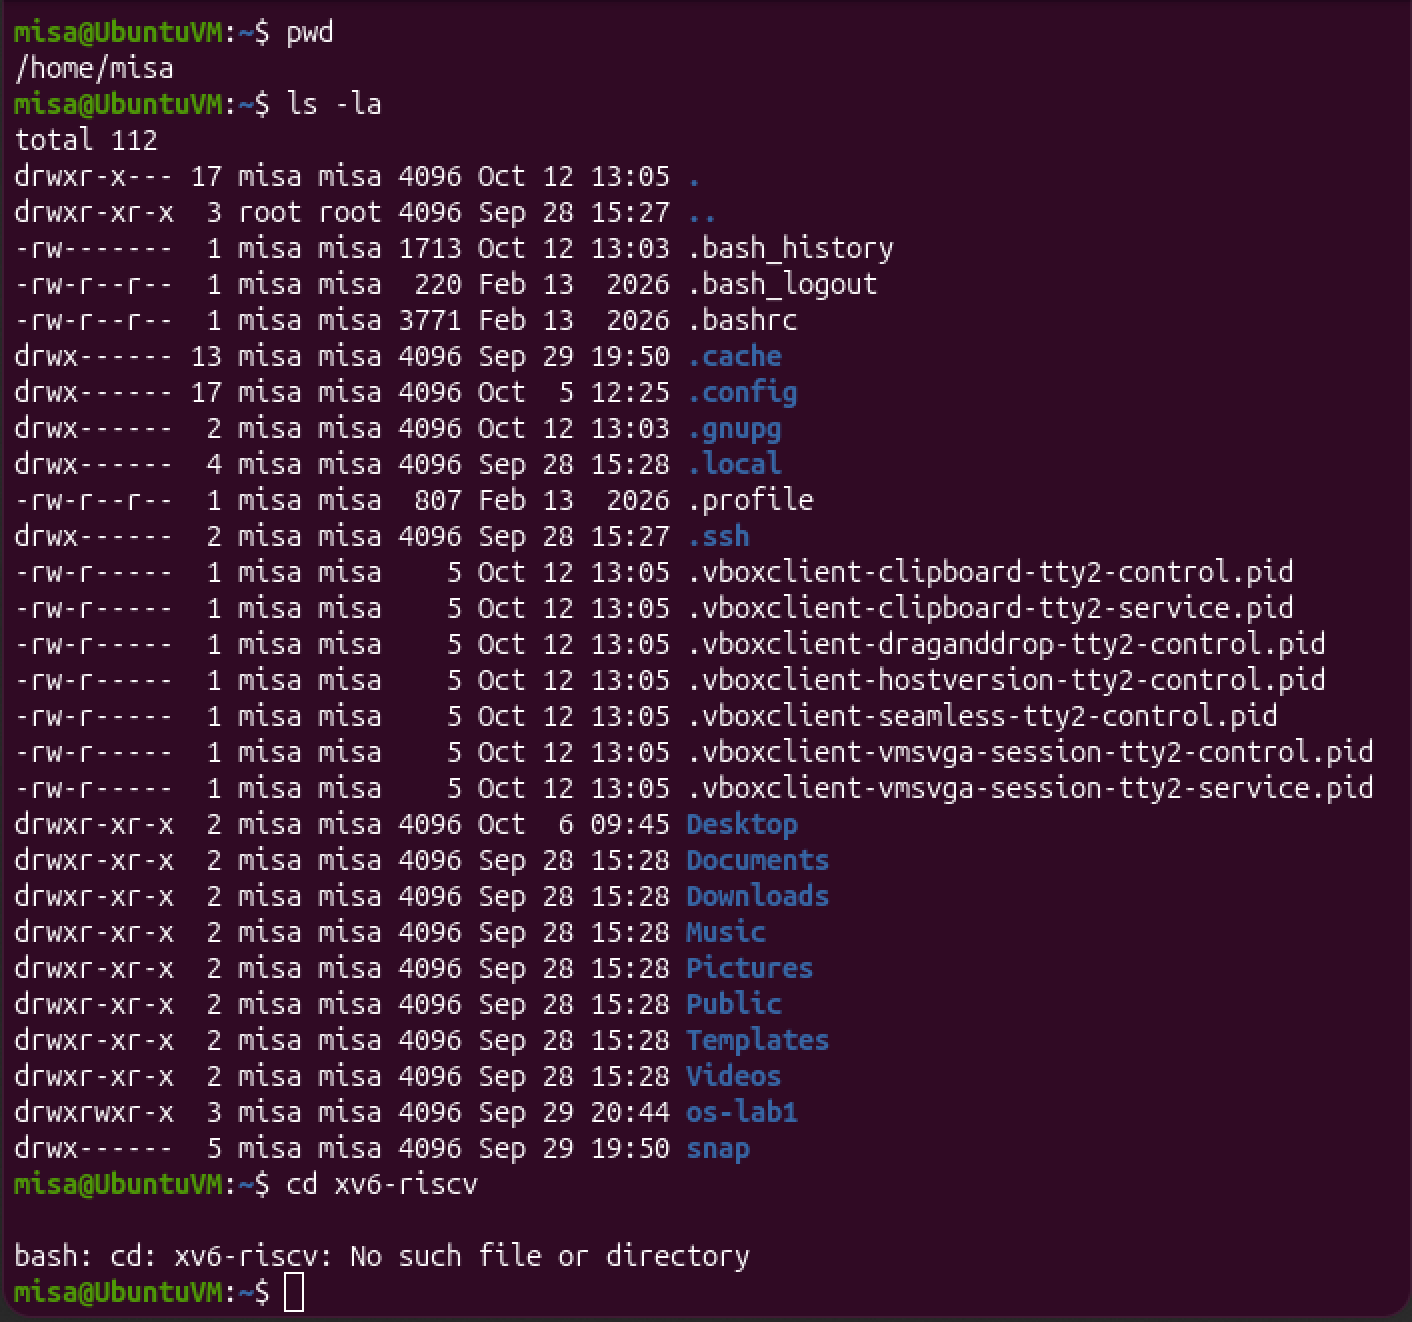
\includegraphics[width=0.82\textwidth]{./img/img_01.png}
    \caption{Checking the home directory for the xv6 source code}
    \label{fig:xv6_directory_check}
\end{figure}

The \texttt{xv6-riscv} directory is not present in the home folder, so the
xv6 source code still needs to be obtained.

Before obtaining the source code, we check whether the tools required to
build and run xv6 are available.

\begin{figure}[H]
    \centering
    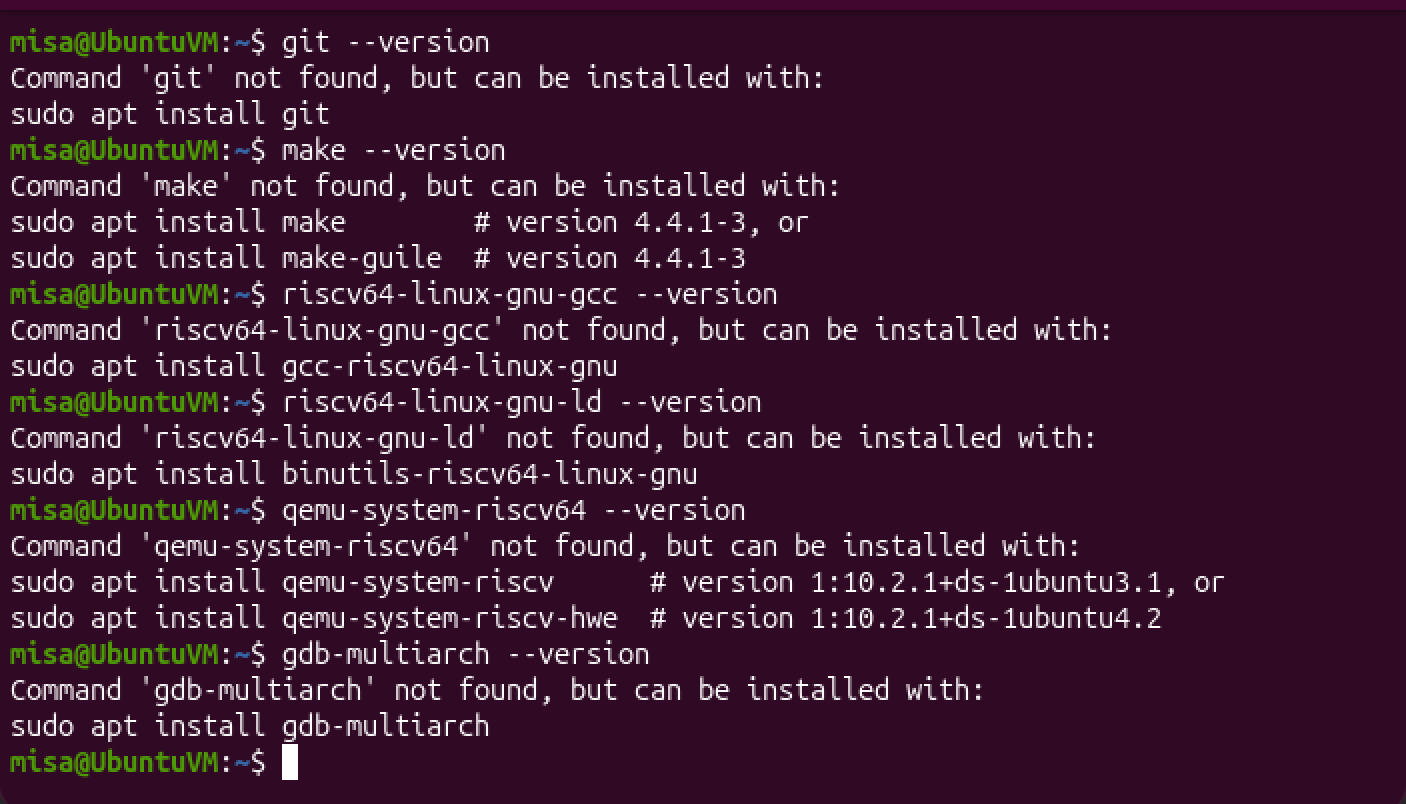
\includegraphics[width=0.82\textwidth]{./img/img_02.png}
    \caption{Checking the availability of the required development tools}
    \label{fig:toolchain_check}
\end{figure}

None of the required tools are currently available in the system. The
development environment therefore needs to be prepared before xv6 can be
built and executed.

The missing tools are installed through the Ubuntu package manager.

\begin{figure}[H]
    \centering
    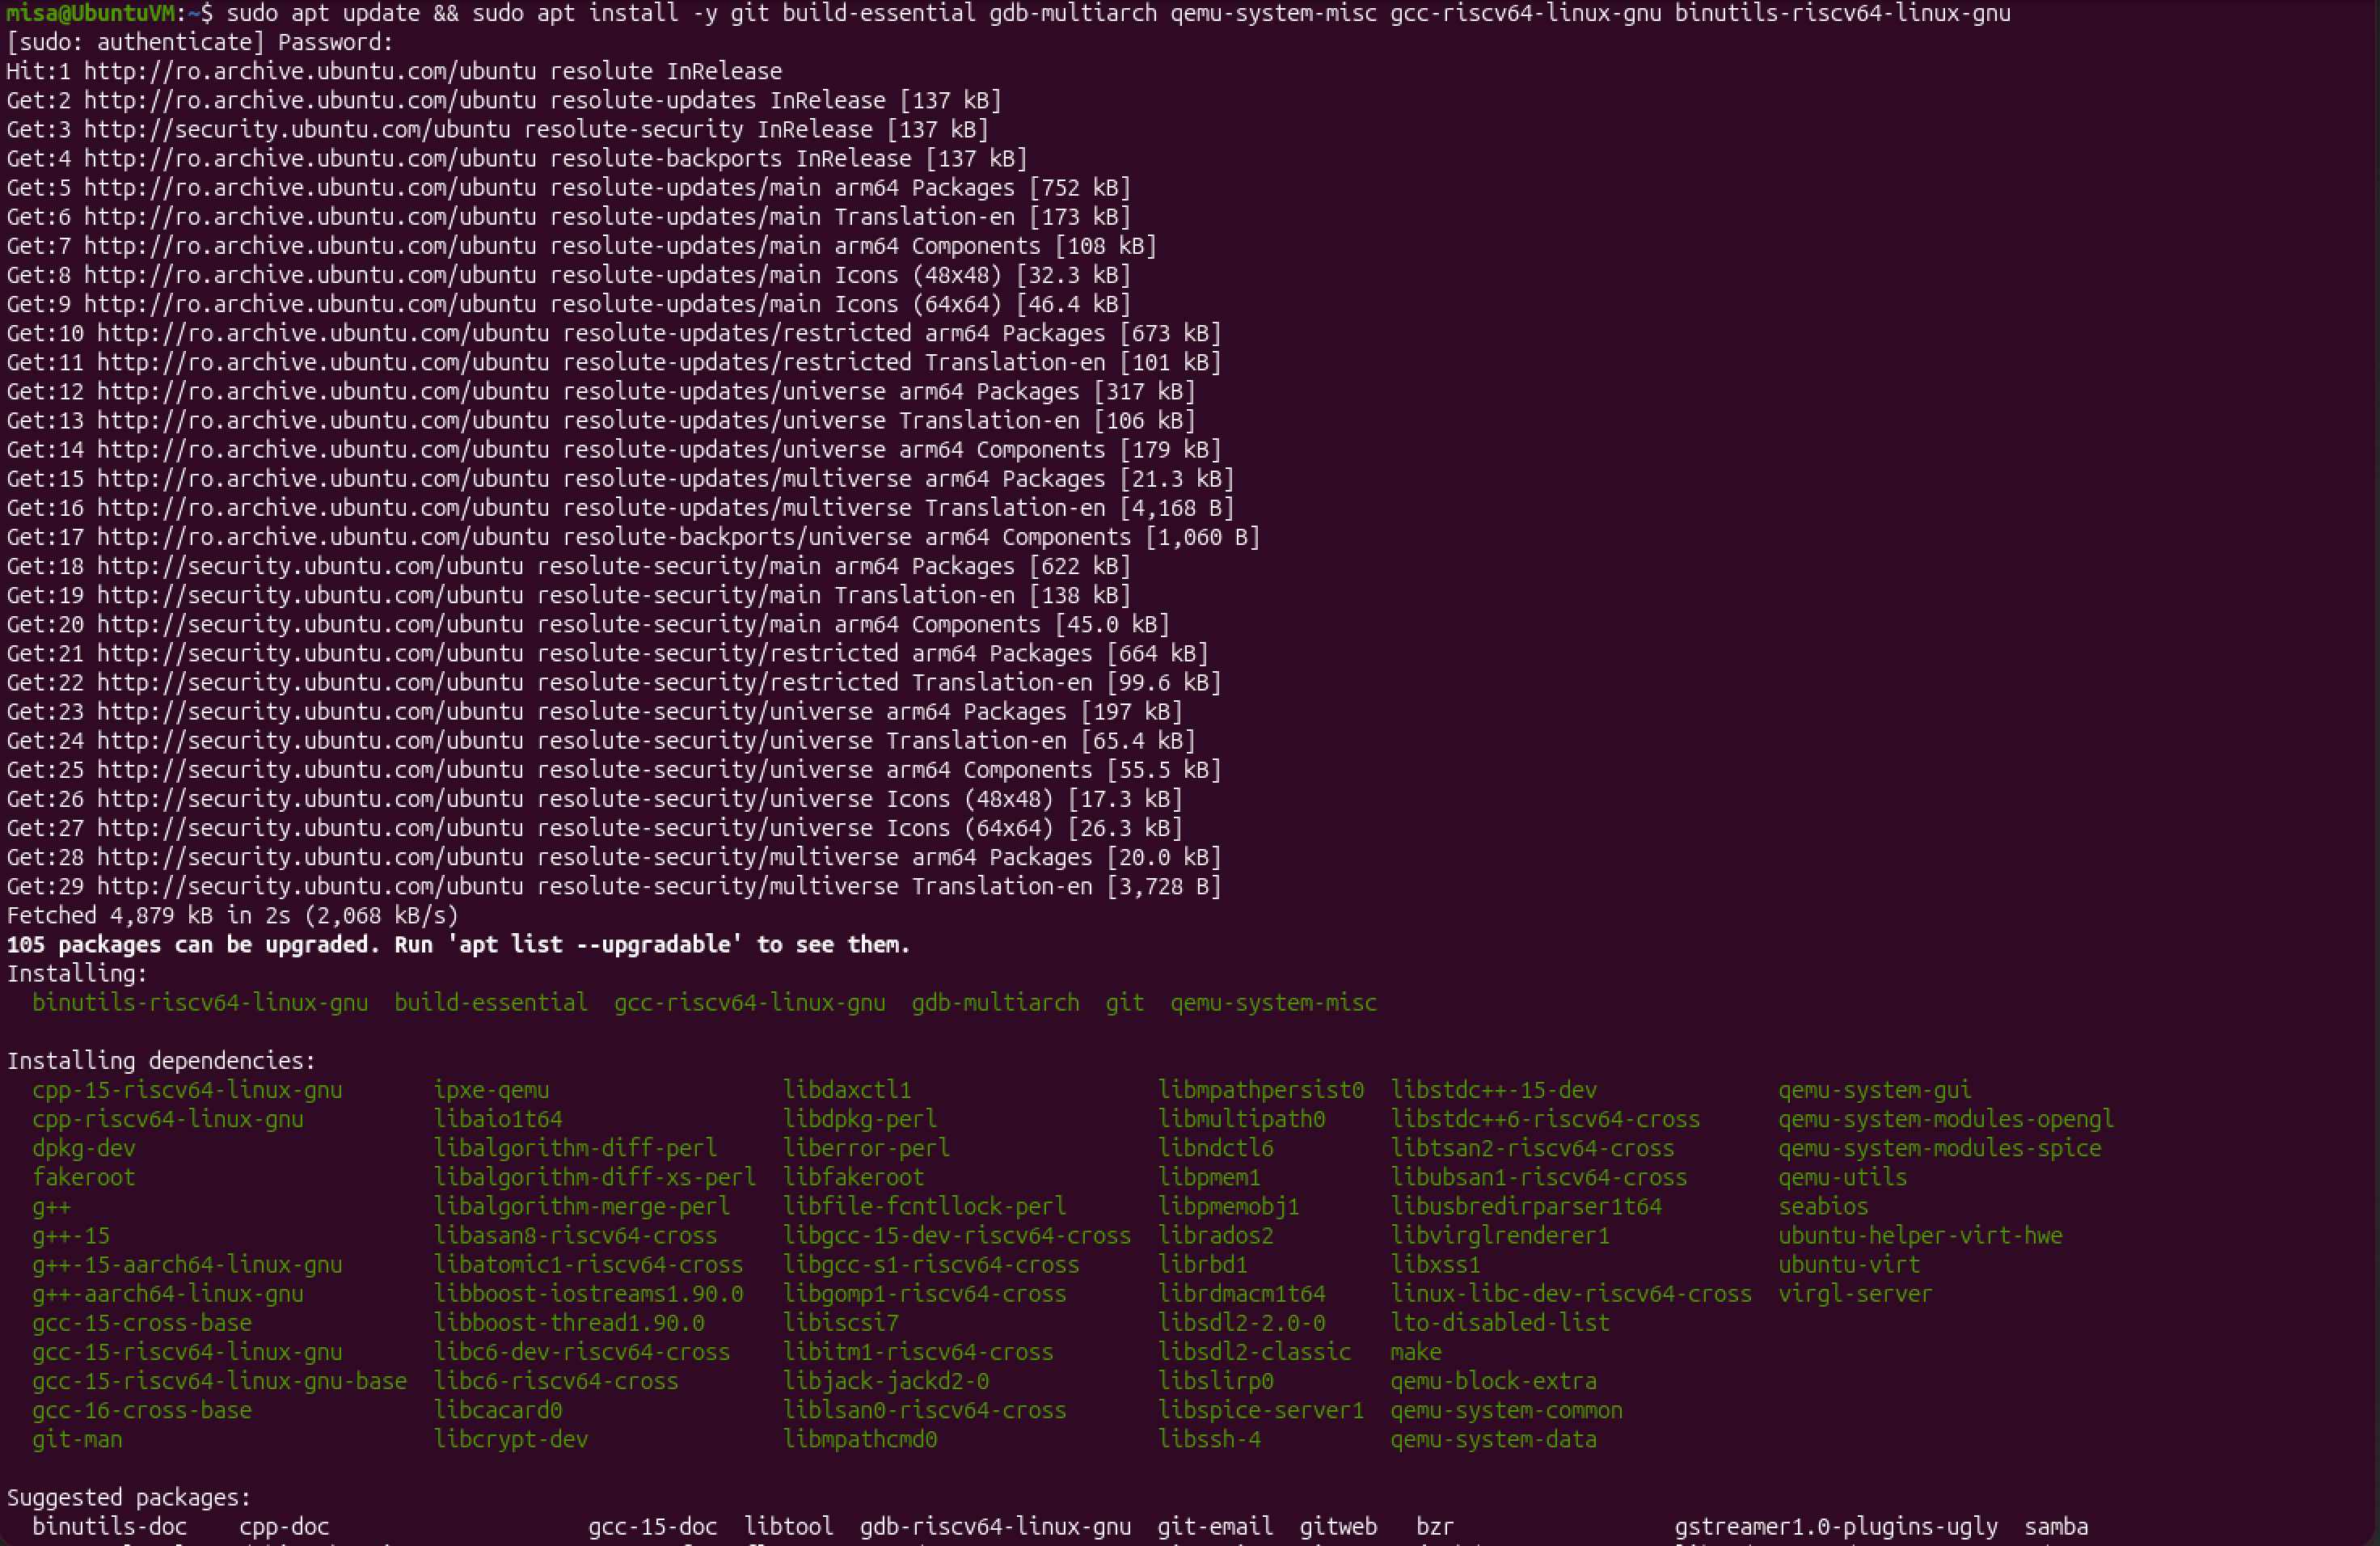
\includegraphics[width=0.82\textwidth]{./img/img_03.png}
    \caption{Installing the xv6 development toolchain}
    \label{fig:toolchain_installation}
\end{figure}

The installed tools were then checked again.

\begin{figure}[H]
    \centering
    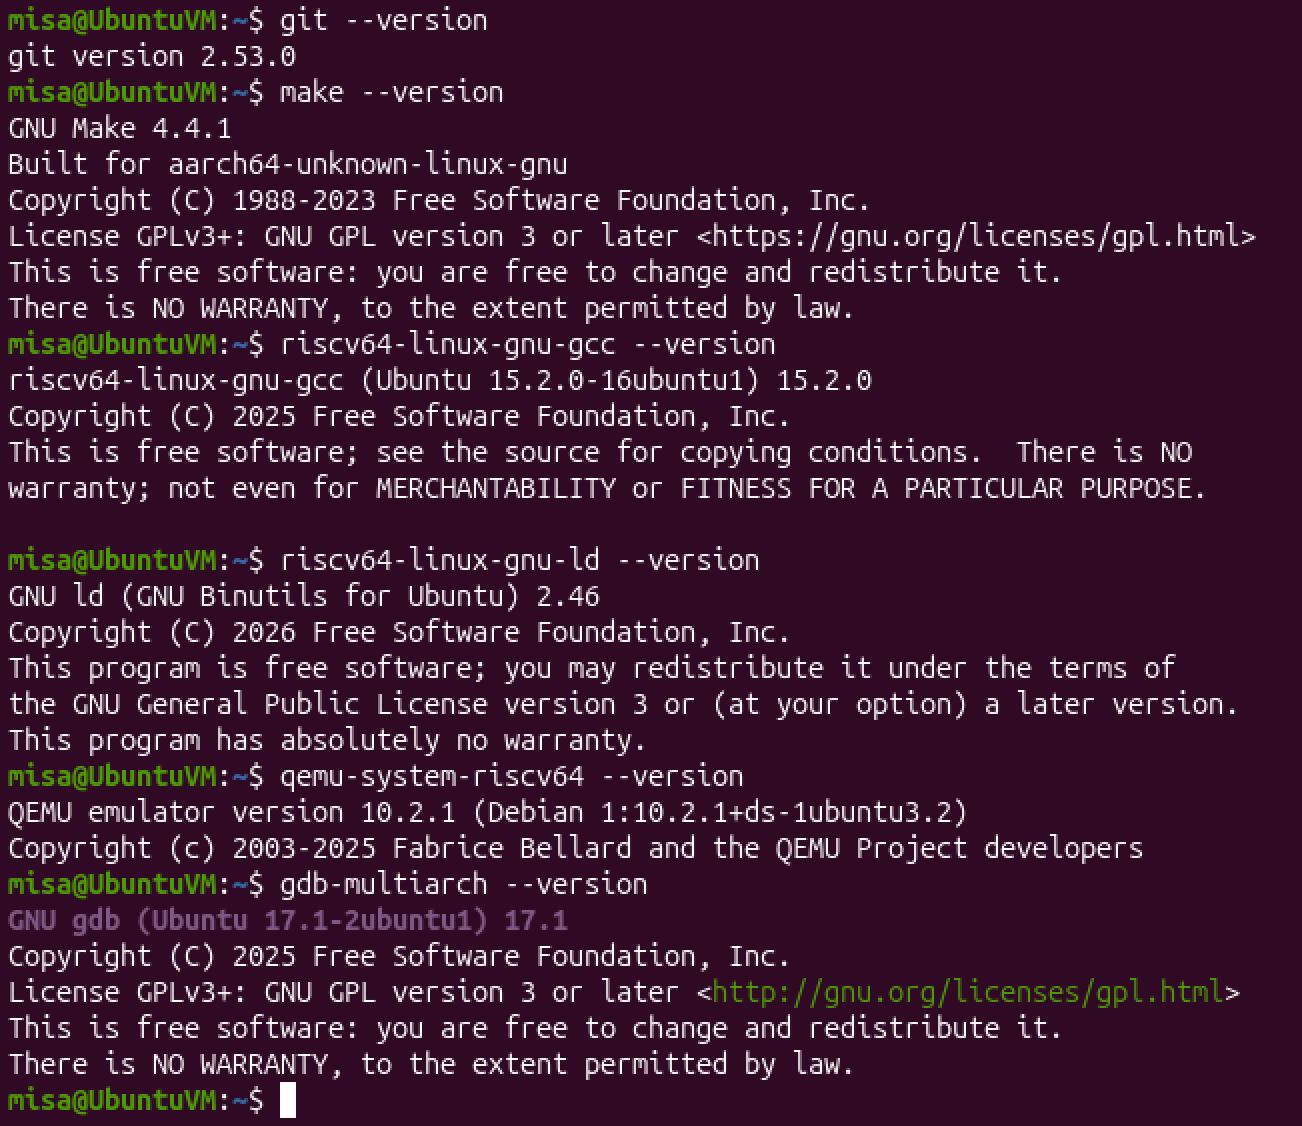
\includegraphics[width=0.82\textwidth]{./img/img_04.png}
    \caption{Verification of the installed development tools}
    \label{fig:toolchain_verification}
\end{figure}

All required development tools are now installed and available in the system.
The environment is ready for working with xv6.

With the development environment ready, the xv6 source code can now be
obtained from the official repository.

\begin{figure}[H]
    \centering
    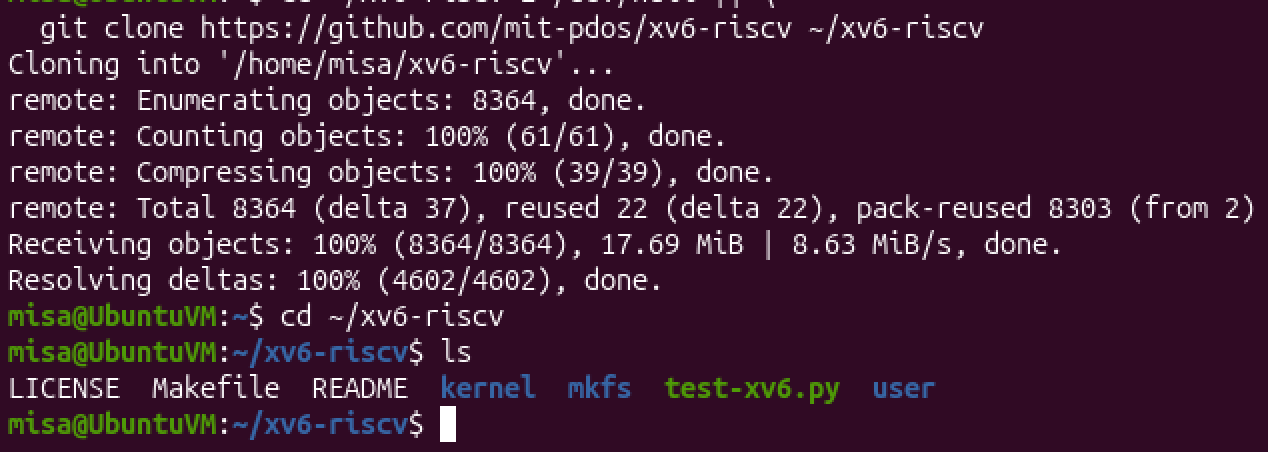
\includegraphics[width=0.82\textwidth]{./img/img_05.png}
    \caption{Cloning and inspecting the xv6 source repository}
    \label{fig:xv6_repository}
\end{figure}

The xv6 source tree is now available in
\texttt{\textasciitilde/xv6-riscv}. It contains the kernel sources, user
programs, the Makefile, and the other files required to build the system.


\chapter{Building the OS}
\section{Build it and boot it}

The xv6 kernel and user programs were built from source using the RISC-V
toolchain. Make compiled and linked the required components, created the
filesystem image, and launched the resulting system in QEMU.

\begin{figure}[H]
    \centering
    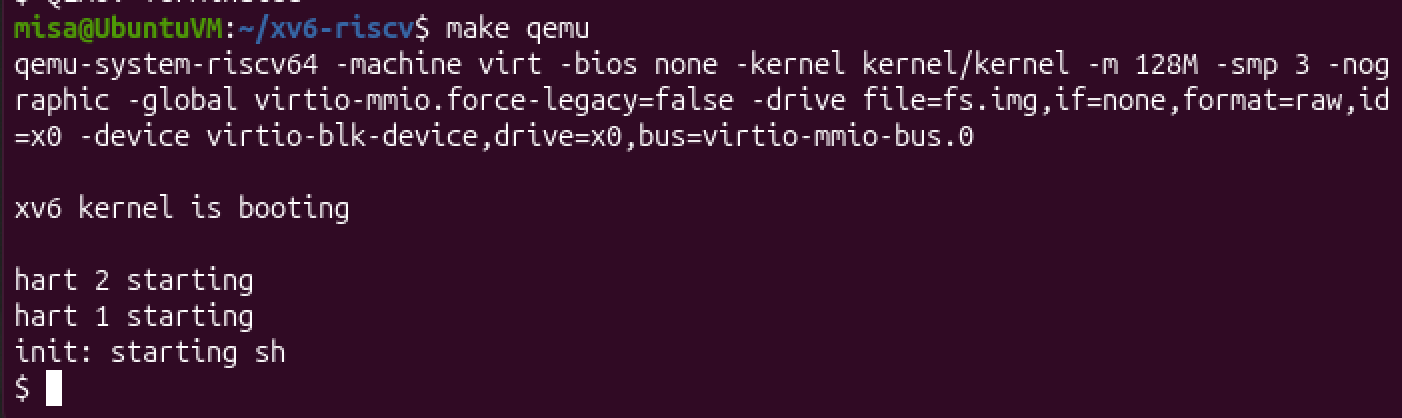
\includegraphics[width=0.82\textwidth]{./img/img_06.png}
    \caption{Booting xv6 in the QEMU RISC-V emulator}
    \label{fig:xv6_boot}
\end{figure}

The boot completed successfully. After initializing the system, xv6 started
its shell and presented the command prompt.



\section{Use xv6 as the Unix it is}

After booting, xv6 provides a simple Unix shell through which user programs
can be executed. Its command interface resembles that of Linux, although
the number of available programs and supported features is considerably
smaller.

We begin by examining the contents of the xv6 filesystem using
\texttt{ls}. The command lists files and directories together with their
types, inode numbers, and sizes in bytes. The output includes familiar
Unix utilities such as \texttt{cat}, \texttt{echo}, \texttt{grep},
\texttt{ls}, and \texttt{wc}, as well as several programs for testing
the operating system.

\begin{figure}[H]
    \centering
    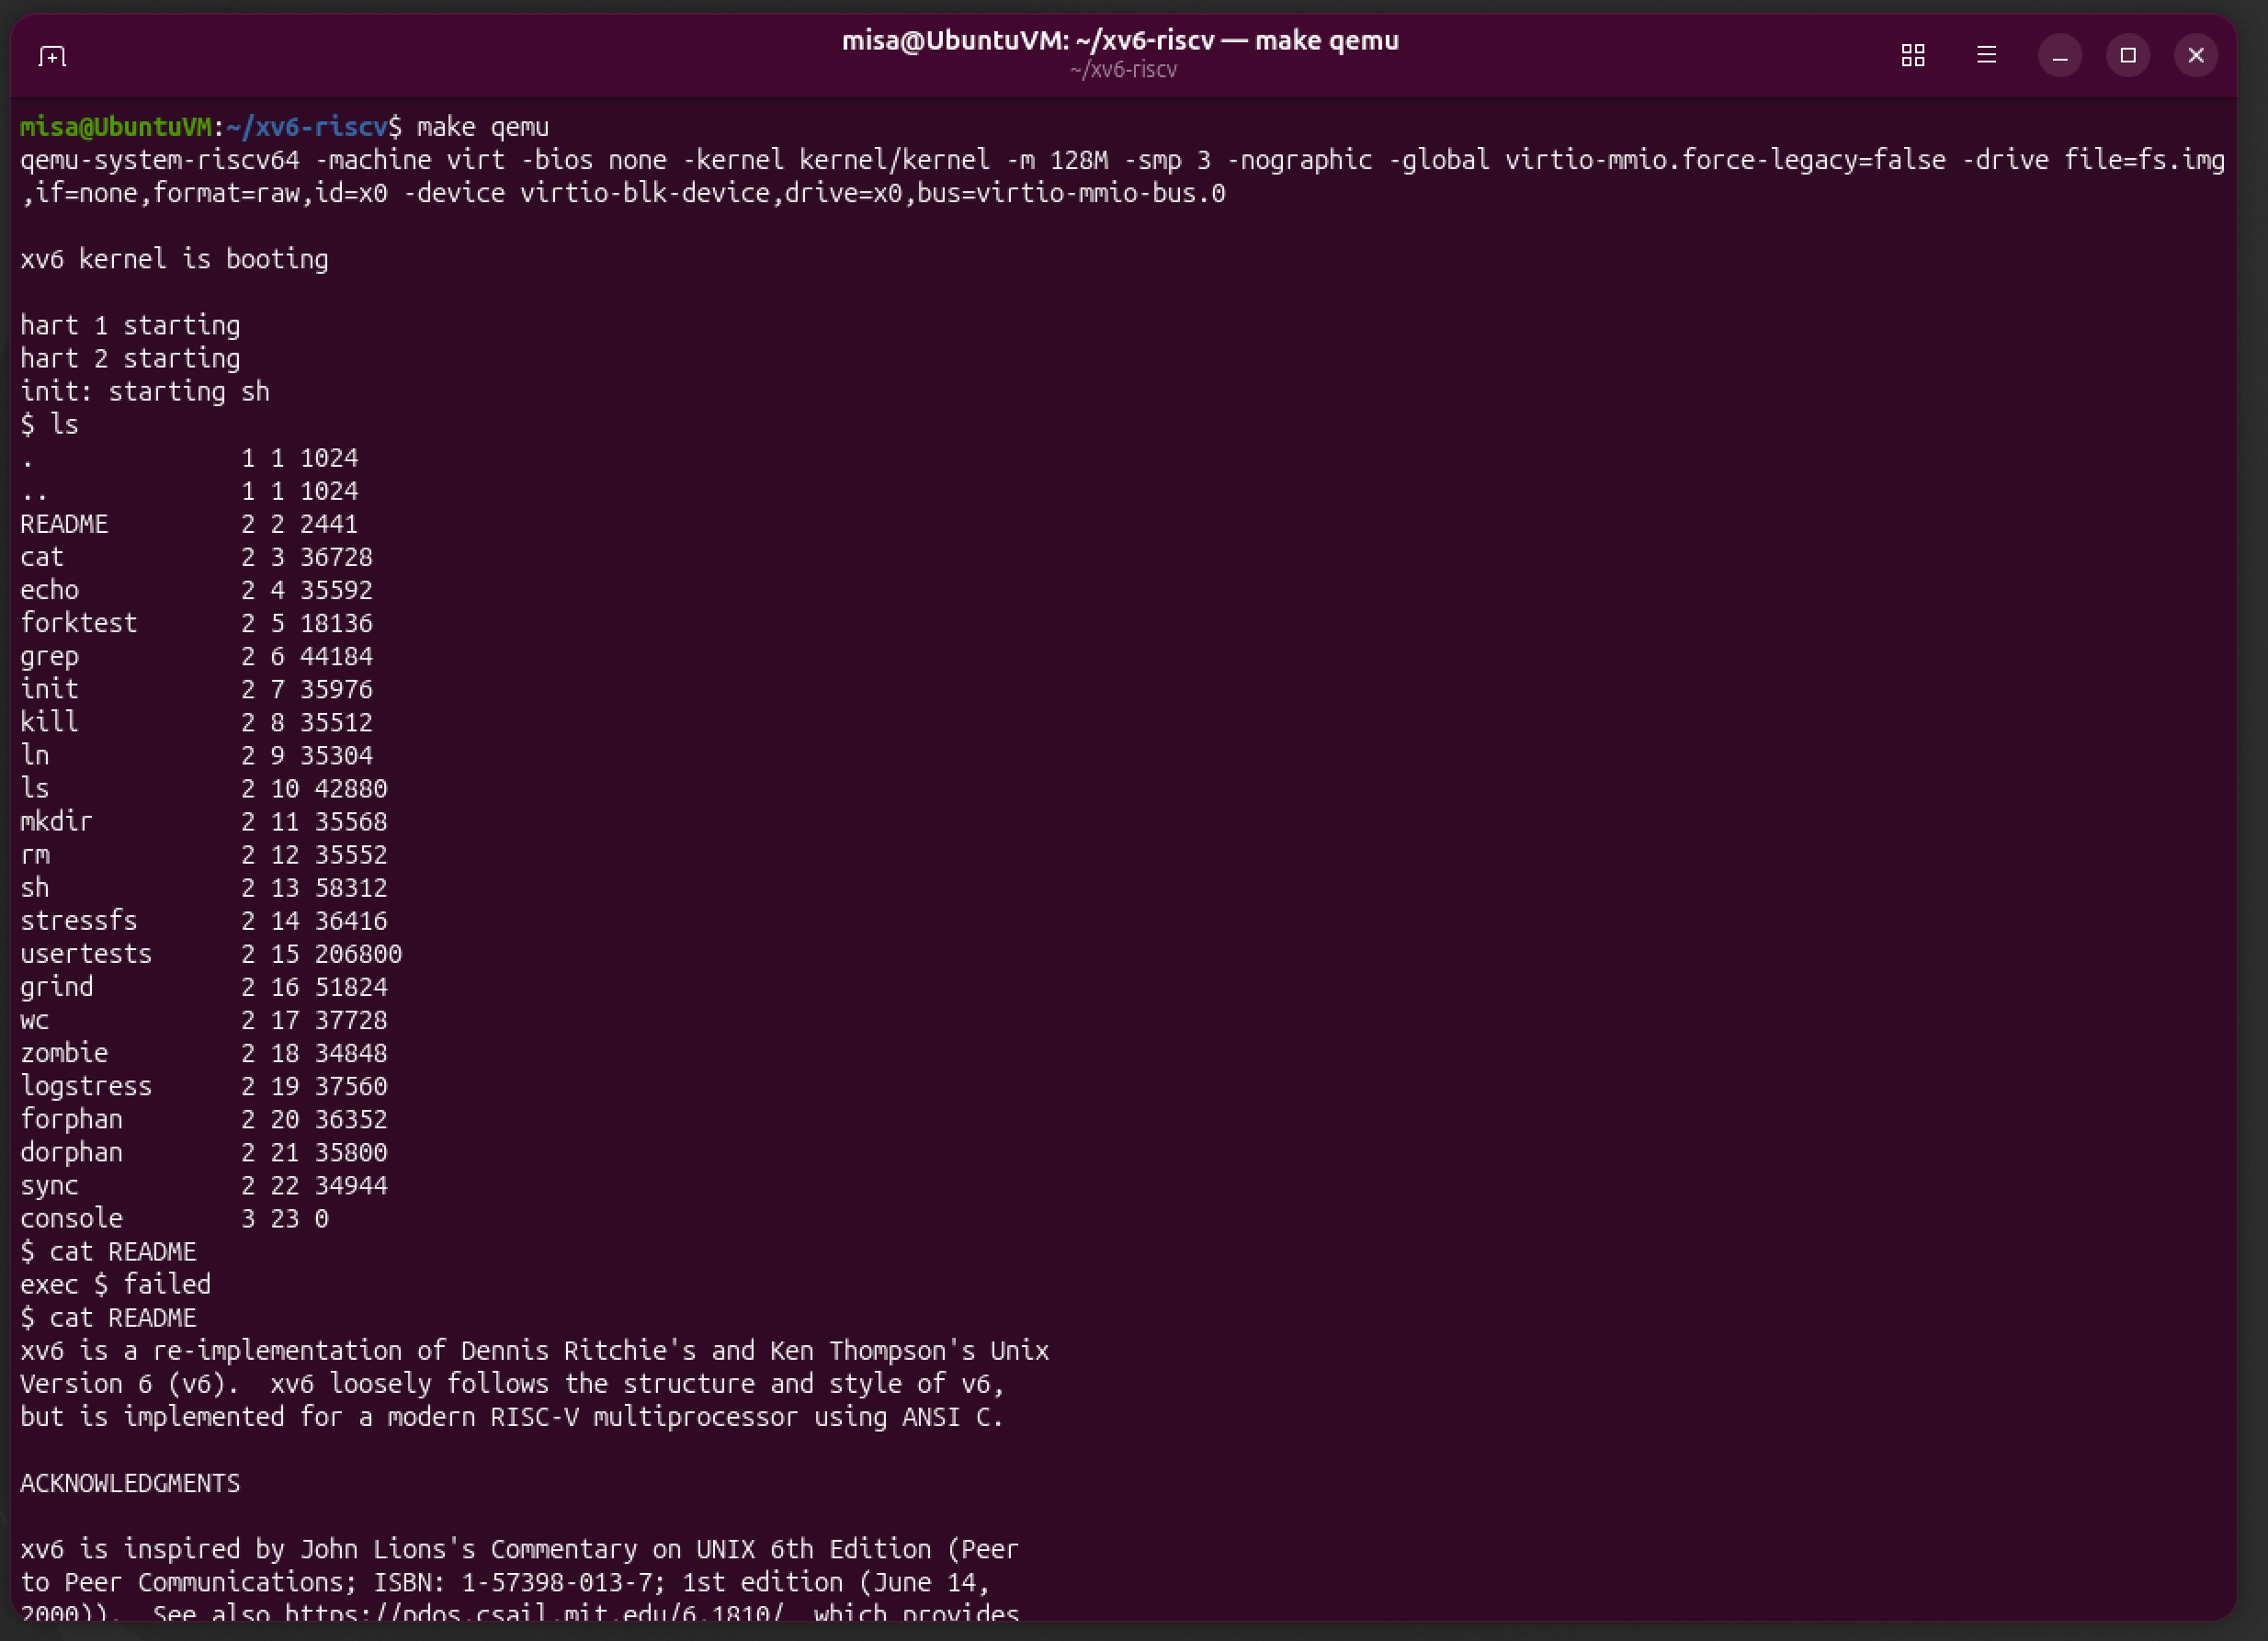
\includegraphics[width=0.82\textwidth]{./img/img_07.png}
    \caption{Exploring the xv6 filesystem using ls}
    \label{fig:xv6_ls}
\end{figure}

The \texttt{README} file is then examined using \texttt{cat}, which
reads a file and writes its contents to standard output. The file
describes the origins of xv6, acknowledges its contributors, and
provides information about building and running the system.

\begin{figure}[H]
    \centering
    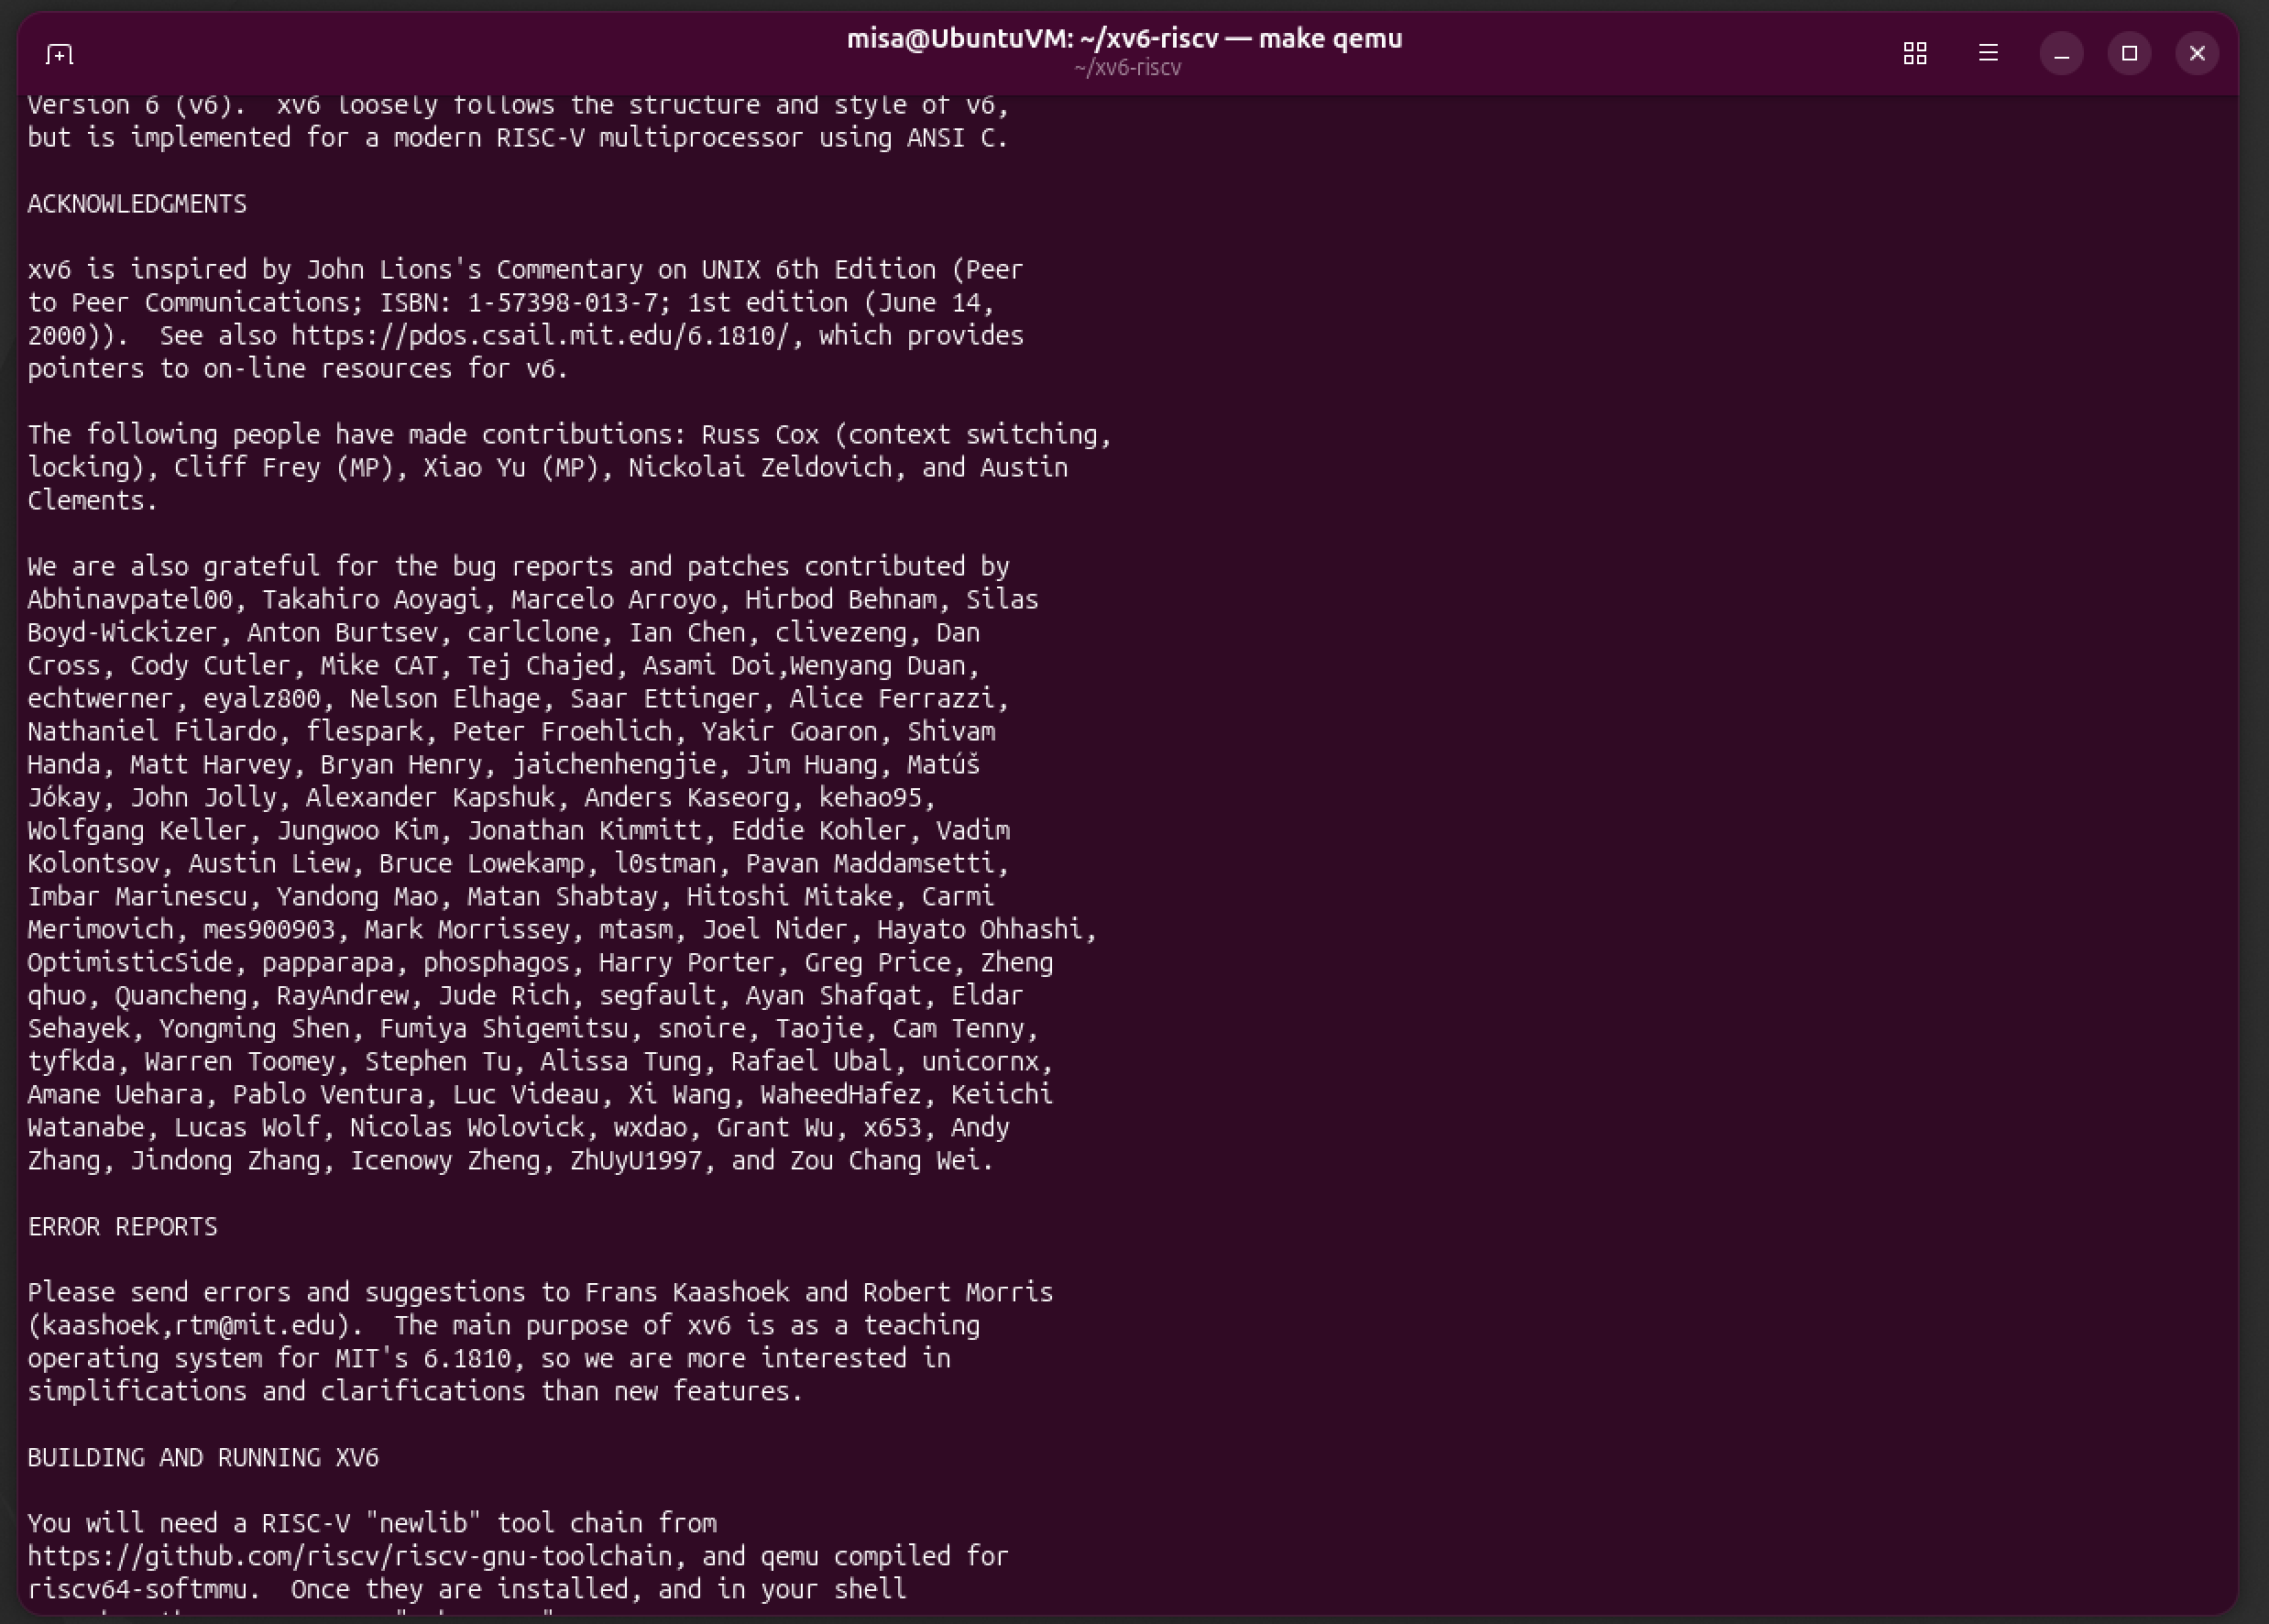
\includegraphics[width=0.82\textwidth]{./img/img_08.png}
    \caption{Reading the xv6 README file}
    \label{fig:xv6_readme}
\end{figure}

The \texttt{echo} command demonstrates basic terminal output by printing
the supplied arguments. Executing it with the words
\texttt{hello xv6} produces the corresponding text in the terminal.

Next, a pipeline is tested using \texttt{ls | grep c}.
The \texttt{ls} command generates a directory listing, while
\texttt{grep} searches its input for lines containing a specified
pattern. Here, the pattern is the character \texttt{c}.

The pipe operator \texttt{|} connects the standard output of
\texttt{ls} to the standard input of \texttt{grep}. As a result,
only entries containing the character \texttt{c} are displayed,
including \texttt{cat}, \texttt{echo}, \texttt{wc},
\texttt{sync}, and \texttt{console}.

This demonstrates two important operating system mechanisms:
process management and inter-process communication. The shell
creates processes for the connected programs, while the kernel
provides a pipe through which data can be transferred between them.

The \texttt{wc} utility is then used to examine the
\texttt{README} file. The command counts lines, words, and bytes.
The result shows that the file contains 48 lines, 336 words,
and 2441 bytes.

\begin{figure}[H]
    \centering
    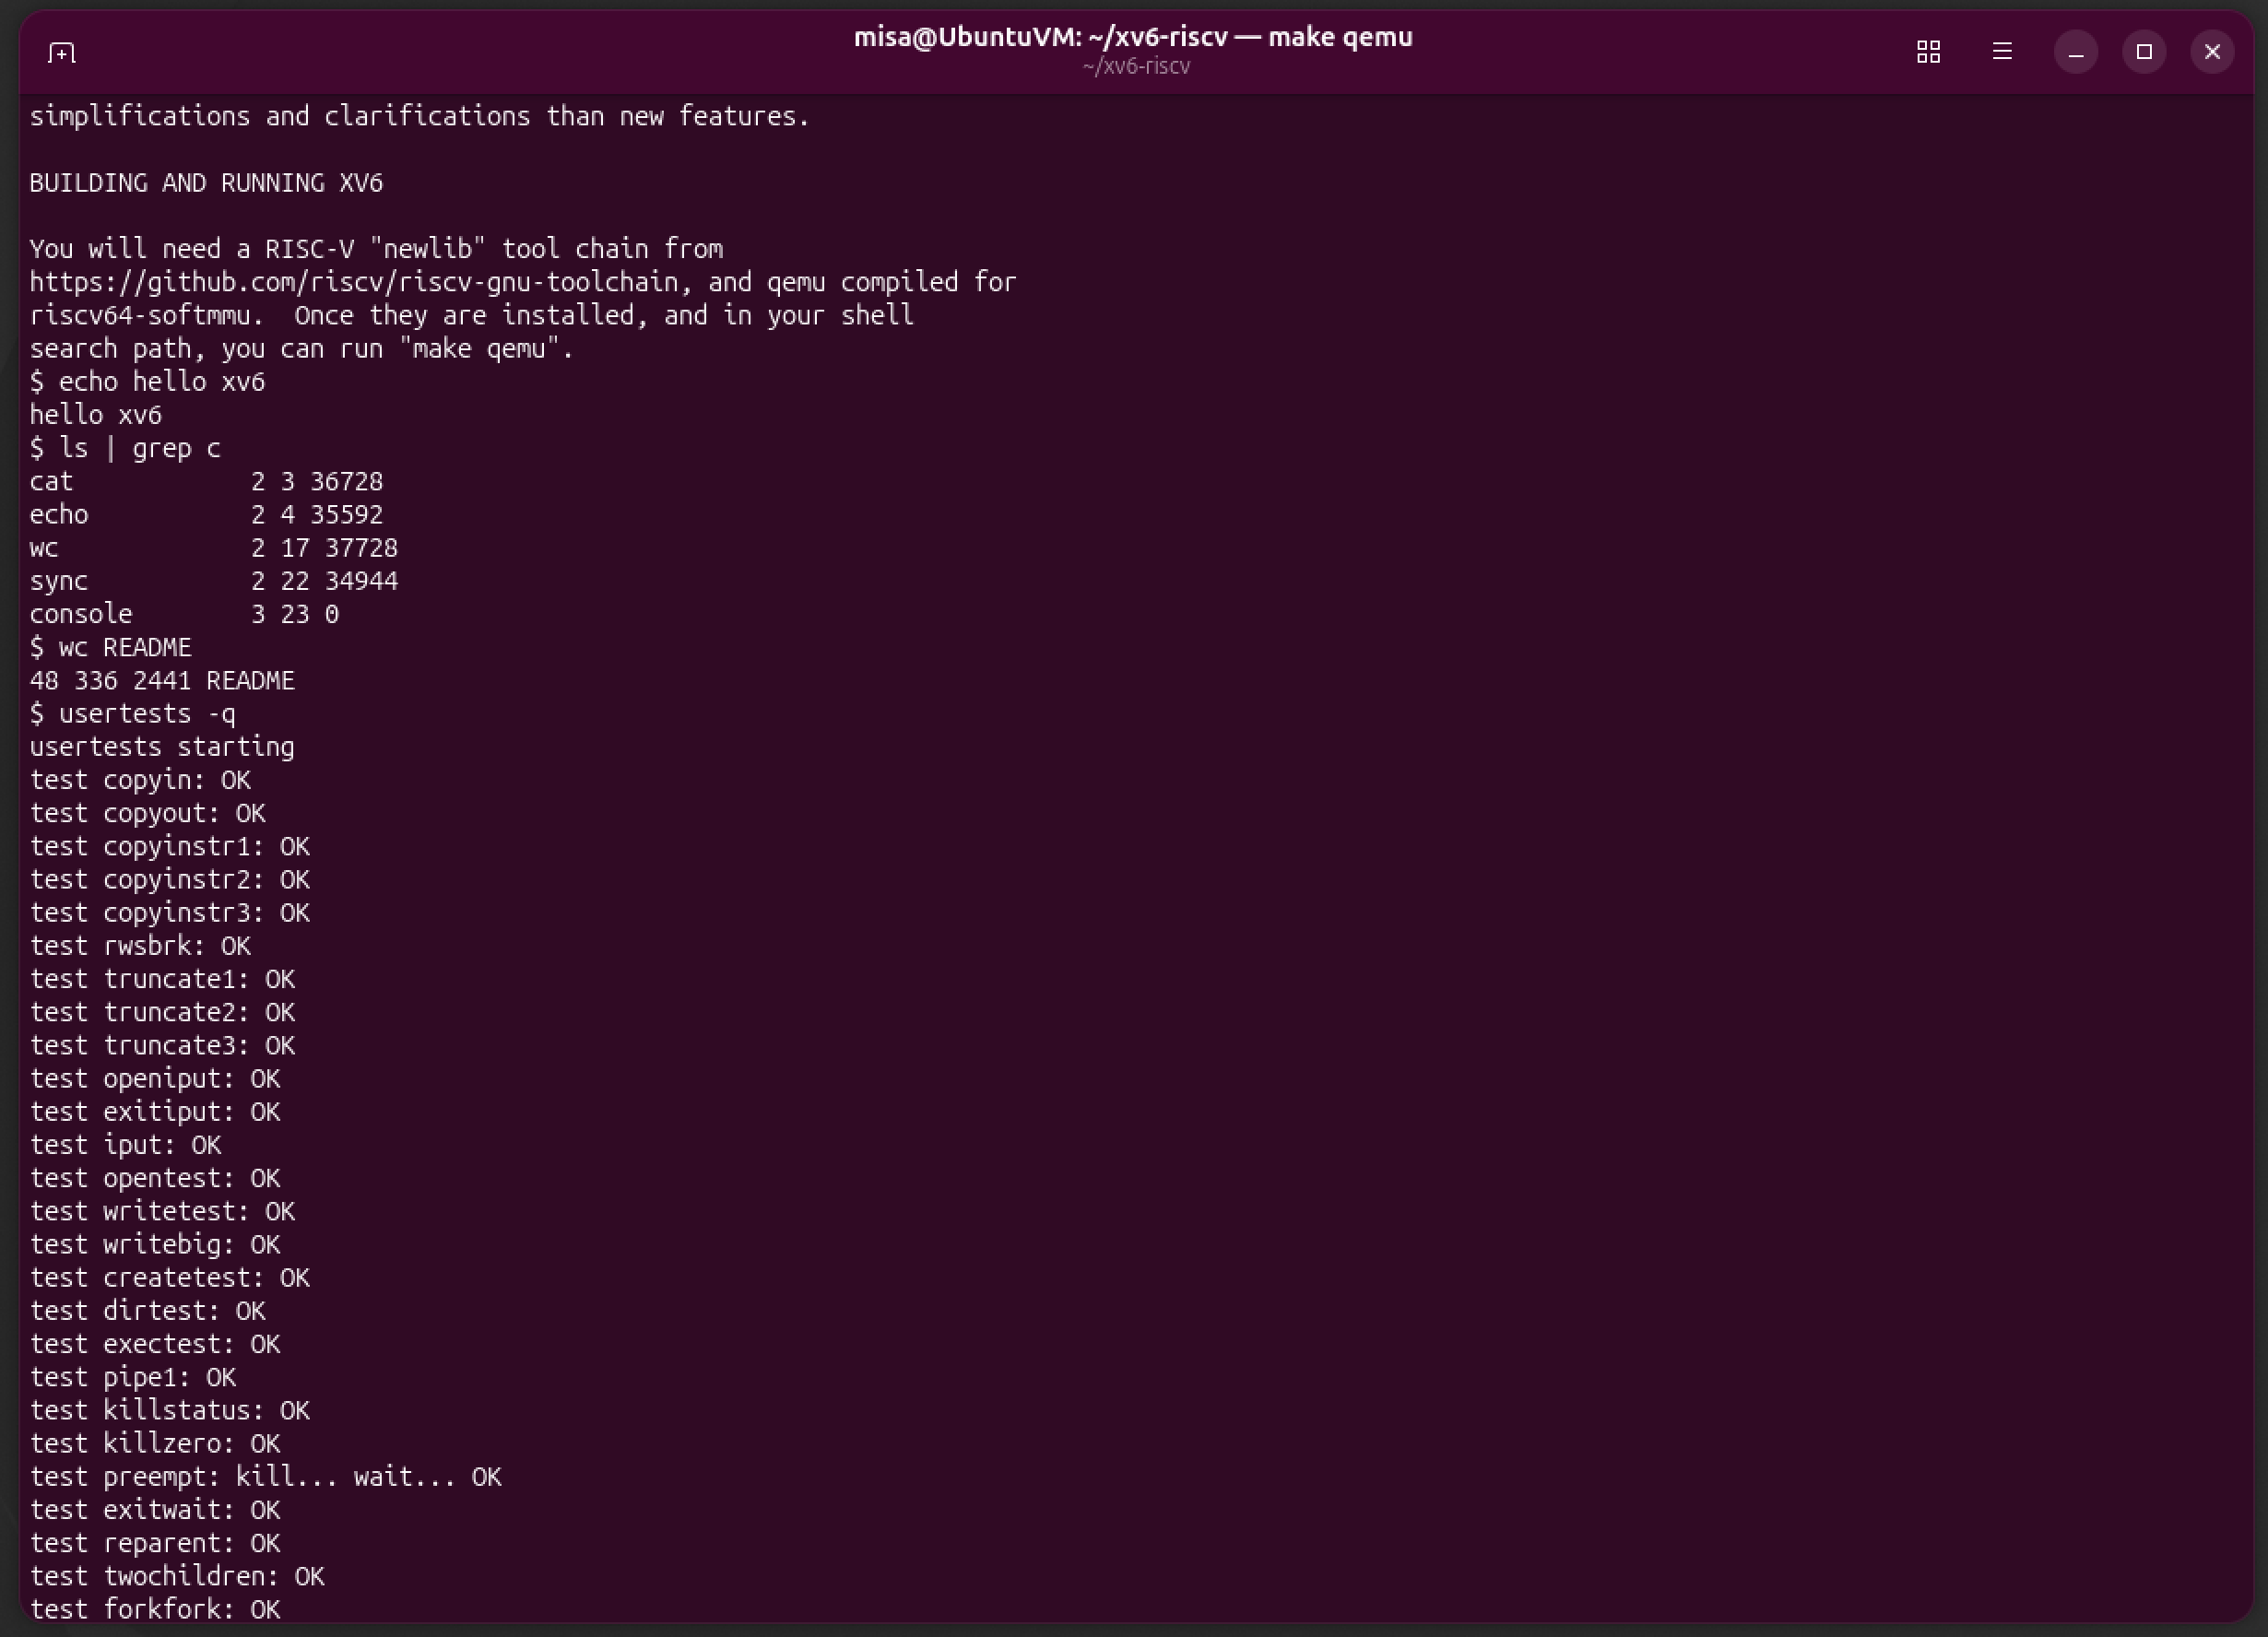
\includegraphics[width=0.82\textwidth]{./img/img_09.png}
    \caption{Testing shell commands, pipelines, and file statistics}
    \label{fig:xv6_shell_commands}
\end{figure}

Finally, the operating system is tested using
\texttt{usertests -q}. The \texttt{usertests} program runs
a collection of tests covering various kernel services,
including process management, memory allocation, filesystem
operations, and system calls.

The \texttt{-q} option enables quiet mode, suppressing some
of the detailed progress messages produced by the test suite.
Individual test results are still displayed.

During execution, several tests deliberately trigger exceptions
to verify how the kernel handles invalid memory accesses and
other exceptional conditions. These produce diagnostic messages
such as \texttt{usertrap(): unexpected scause}, followed by
the corresponding test results.

The test suite completes with the message
\texttt{ALL TESTS PASSED}, confirming that all executed tests
finished successfully.

\begin{figure}[H]
    \centering
    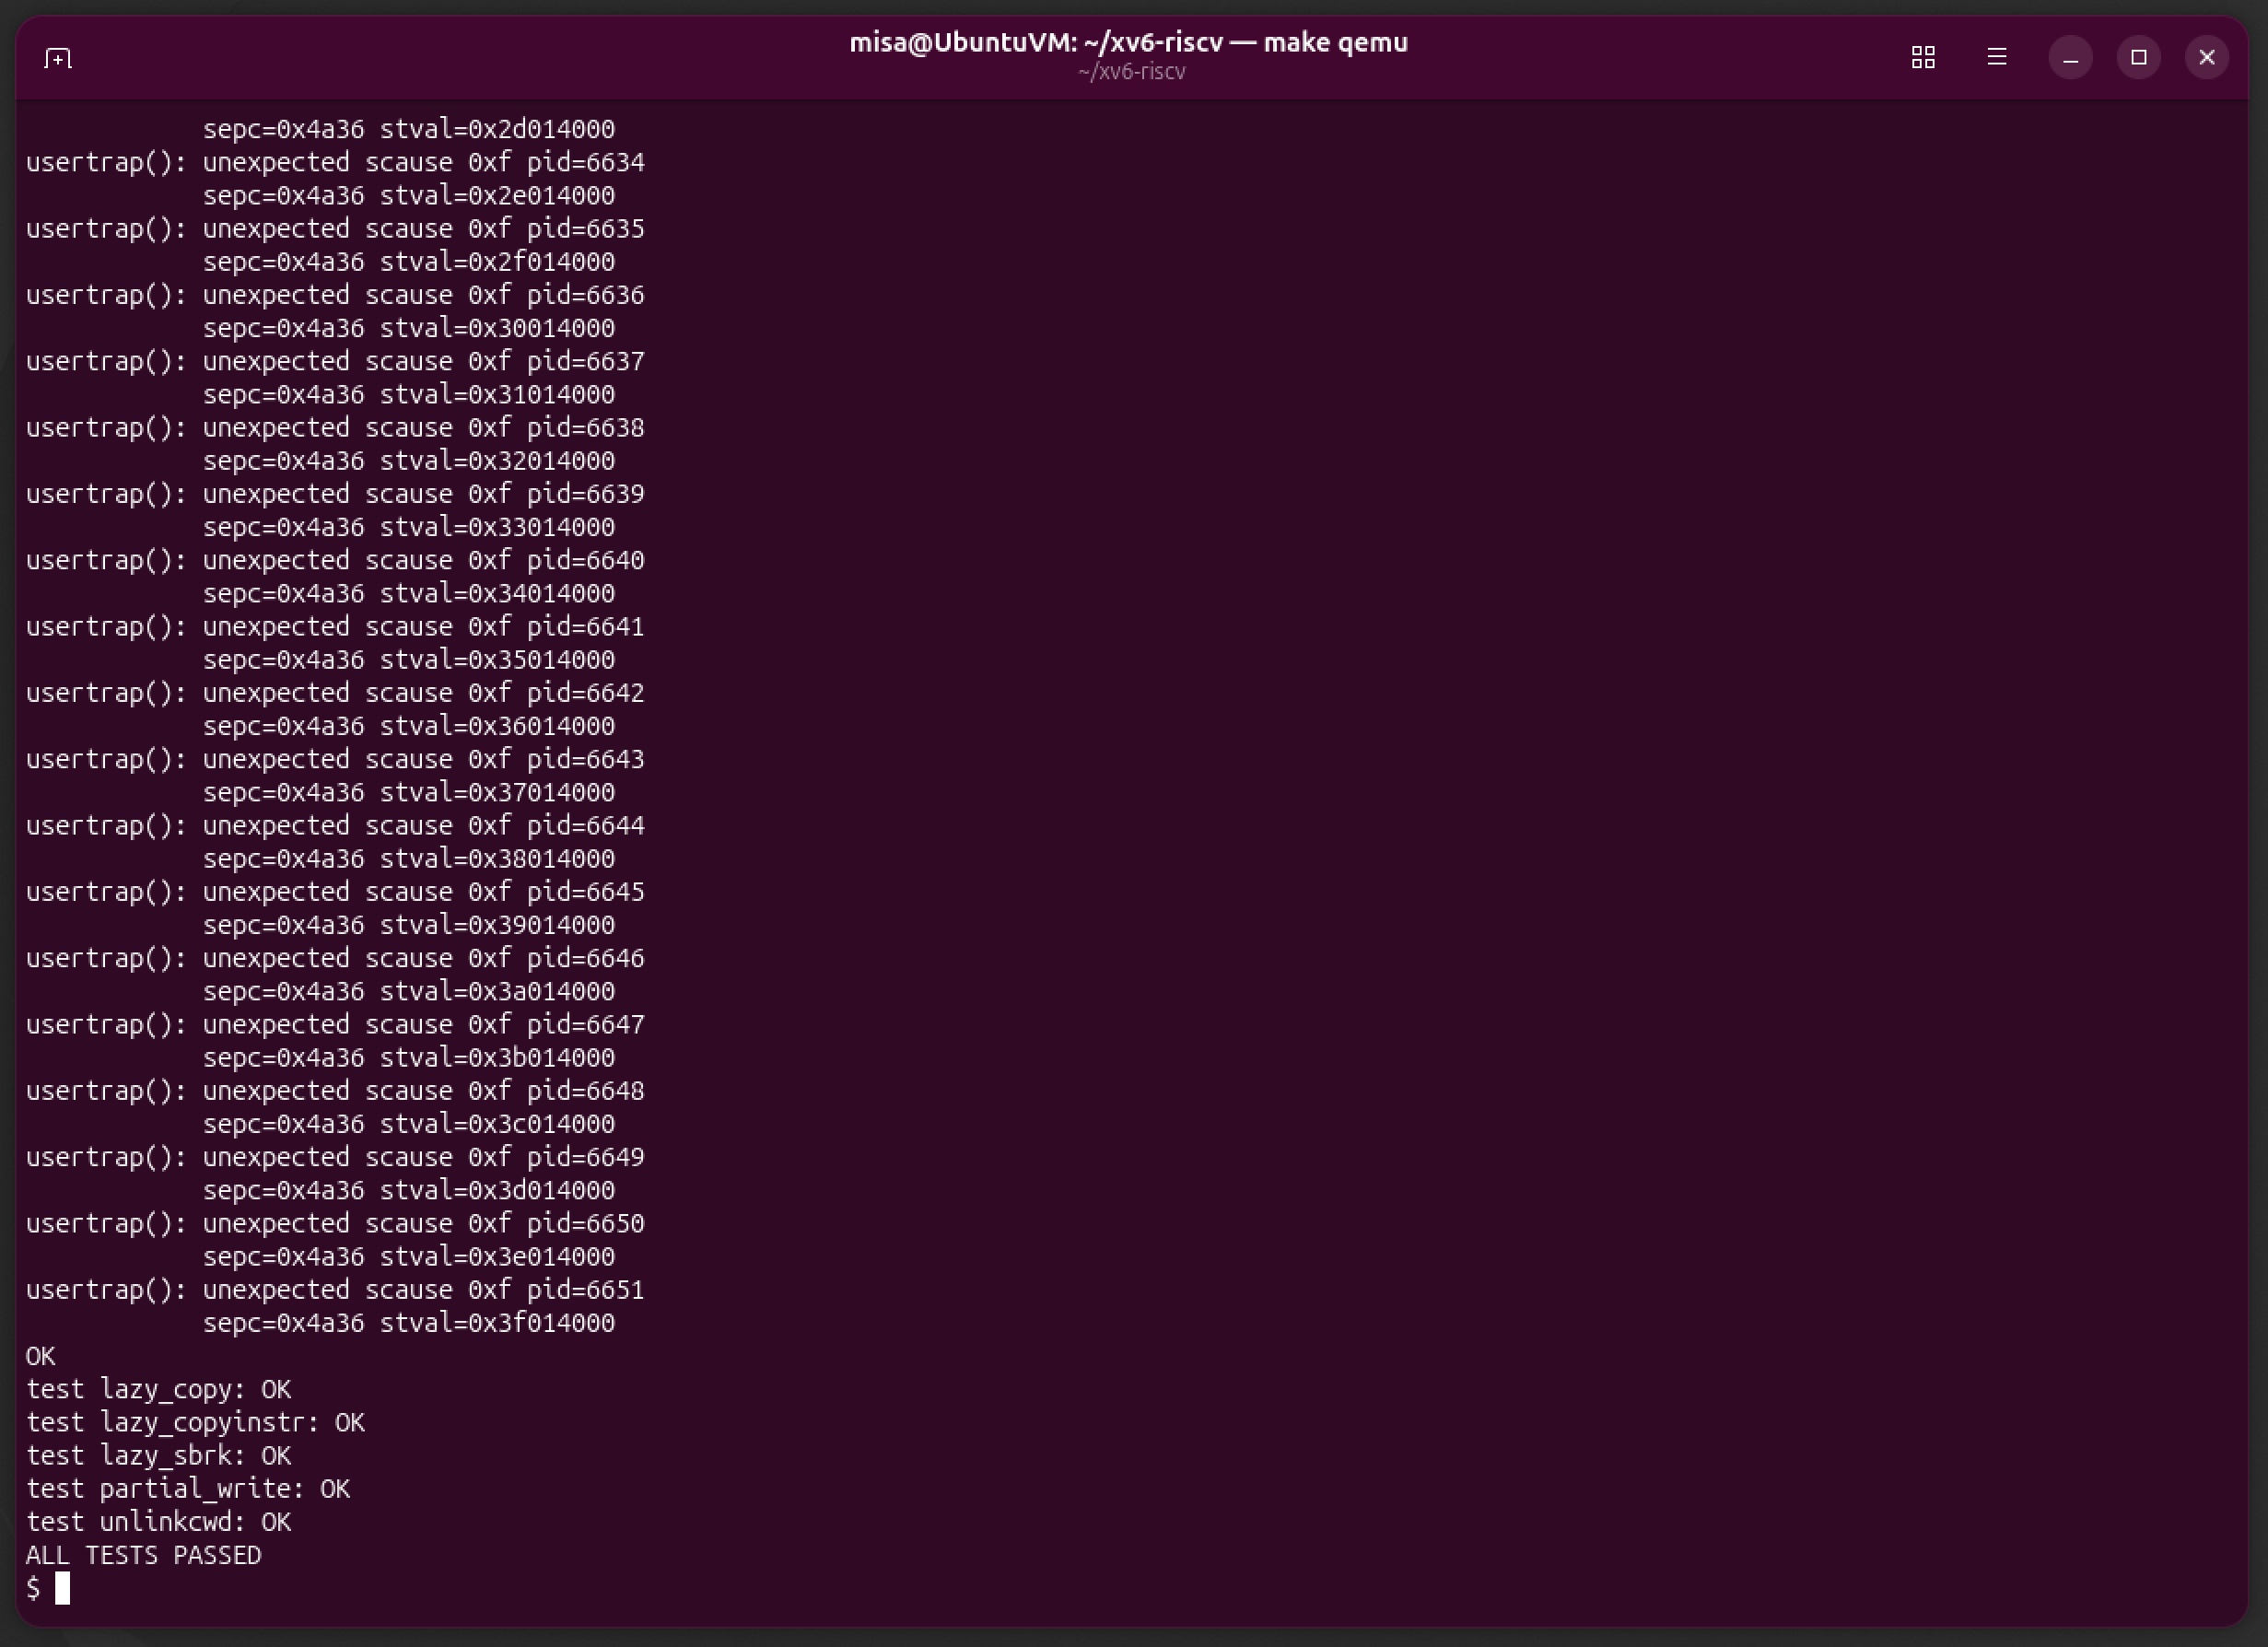
\includegraphics[width=0.82\textwidth]{./img/img_10.png}
    \caption{Successful completion of the xv6 user test suite}
    \label{fig:xv6_usertests}
\end{figure}

The experiments demonstrate that xv6 supports the fundamental
Unix mechanisms needed to execute user programs, access files,
communicate between processes, and interact through a shell.
Its interface resembles a Linux shell, but provides a smaller
collection of commands and features.


\subsection{Observations}

\begin{enumerate}
    \item \textbf{List three programs xv6 ships with.}

    xv6 includes several standard Unix utilities, including
    \texttt{cat}, \texttt{echo}, and \texttt{grep}.
    These programs are available directly from the xv6 shell.

    \item \textbf{You just used a pipe (\texttt{|}) inside xv6.
    Which two OS features must exist for a pipe to work?}

    A pipeline requires process management and inter-process
    communication (IPC). The operating system must support
    the execution of separate processes and provide a pipe
    through which one process can send data to another.

    \item \textbf{In one sentence: how does the xv6 shell compare
    to the Linux shell from Lab 1?}

    The xv6 shell supports familiar Unix commands and pipelines,
    but provides fewer utilities and features than a modern
    Linux shell.
\end{enumerate}

\section{Read the source}

The xv6 source tree is organized around two main directories:
\texttt{kernel/} and \texttt{user/}. The first contains the operating
system kernel, including process scheduling, memory management,
filesystem operations, and system call handlers. The second contains
user-space programs that rely on the kernel to access operating
system services.

To examine this separation, the source code of two familiar
utilities, \texttt{ls} and \texttt{cat}, was inspected.

The \texttt{sed} utility allows selected portions of a text file
to be displayed. The option \texttt{-n} suppresses automatic printing,
while the expression \texttt{1,40p} prints lines 1 through 40.
This makes it possible to inspect a specific part of a source file
without displaying its entire contents.

The first 40 lines of \texttt{user/ls.c} contain the header
inclusions, the \texttt{fmtname()} function, and the beginning
of \texttt{ls()}.

The \texttt{fmtname()} function extracts the final component
of a file path and prepares it for display. The \texttt{ls()}
function begins by opening the specified path using
\texttt{open()} and obtaining file information through
\texttt{fstat()}.

\begin{figure}[H]
    \centering
    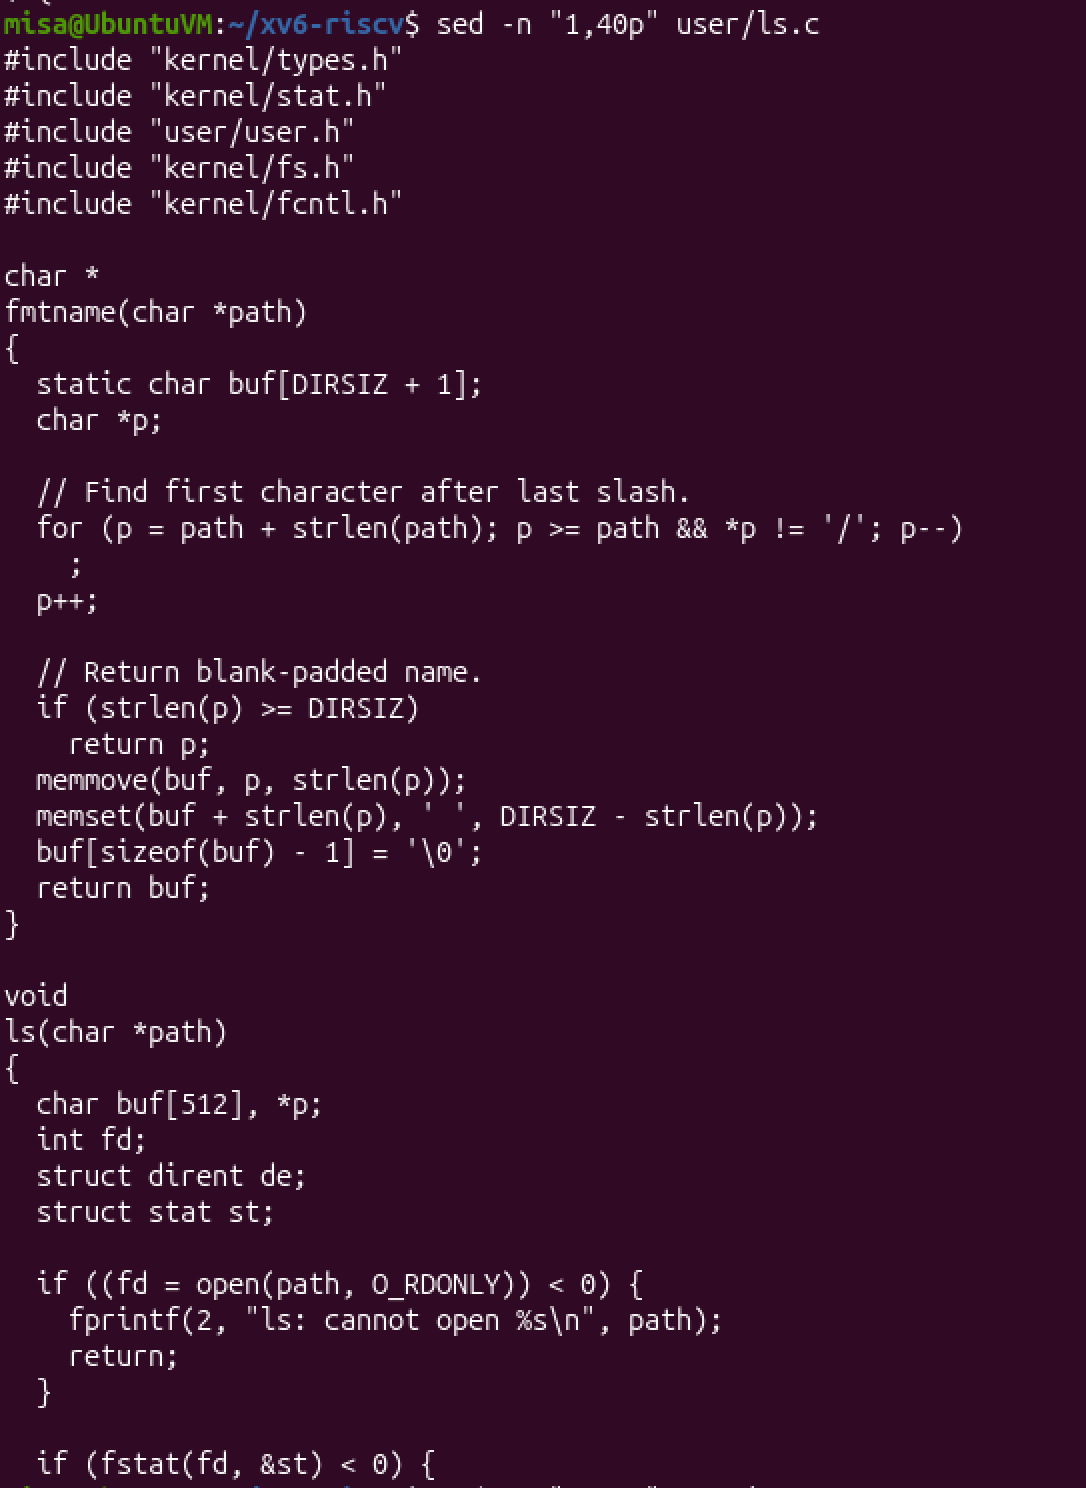
\includegraphics[width=0.82\textwidth]{./img/img_11.png}
    \caption{Examining the source code of the ls utility}
    \label{fig:xv6_ls_source}
\end{figure}

The next program examined is \texttt{user/cat.c}. Its first
30 lines contain a global buffer of 512 bytes and the
\texttt{cat()} function responsible for transferring data
from an input file descriptor to standard output.

The program repeatedly calls \texttt{read()} to obtain data
and \texttt{write()} to send it to the terminal. The loop
continues until \texttt{read()} returns zero, indicating
the end of the input.

The value returned by \texttt{read()} determines how many
bytes are written. A negative return value indicates an
error, while a failed or incomplete write produces an
error message and terminates the program.

The file descriptor passed to \texttt{cat()} identifies the
input source. The value \texttt{1} used in \texttt{write()}
represents standard output, while \texttt{2} used in
\texttt{fprintf()} represents standard error.

\begin{figure}[H]
    \centering
    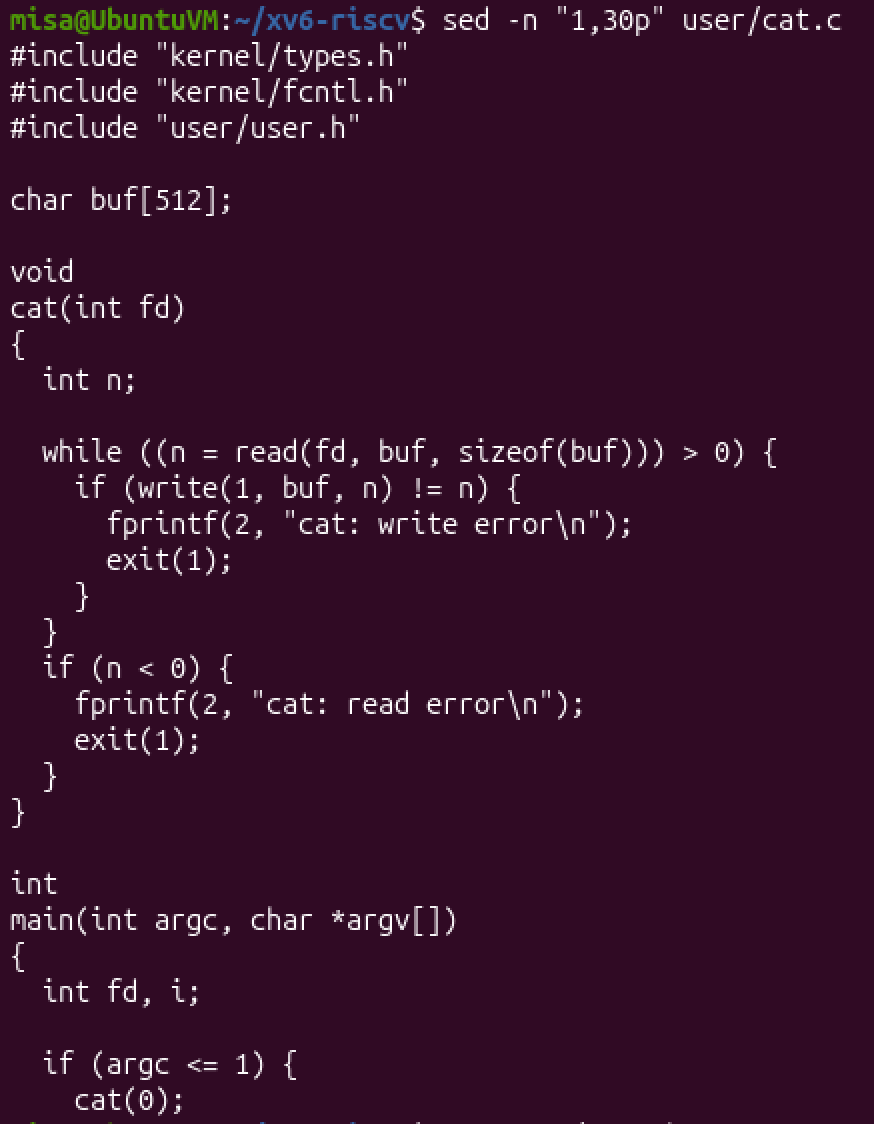
\includegraphics[width=0.82\textwidth]{./img/img_12.png}
    \caption{Examining the source code of the cat utility}
    \label{fig:xv6_cat_source}
\end{figure}

The functions \texttt{read()} and \texttt{write()} provide
an interface between user programs and the operating system
kernel. Their declarations can be found in
\texttt{user/user.h}, together with other system calls
such as \texttt{fork()}, \texttt{exit()}, \texttt{wait()},
\texttt{pipe()}, and \texttt{open()}.

The header also declares ordinary user-space functions,
including string manipulation, memory allocation, and
formatted output routines.

\begin{figure}[H]
    \centering
    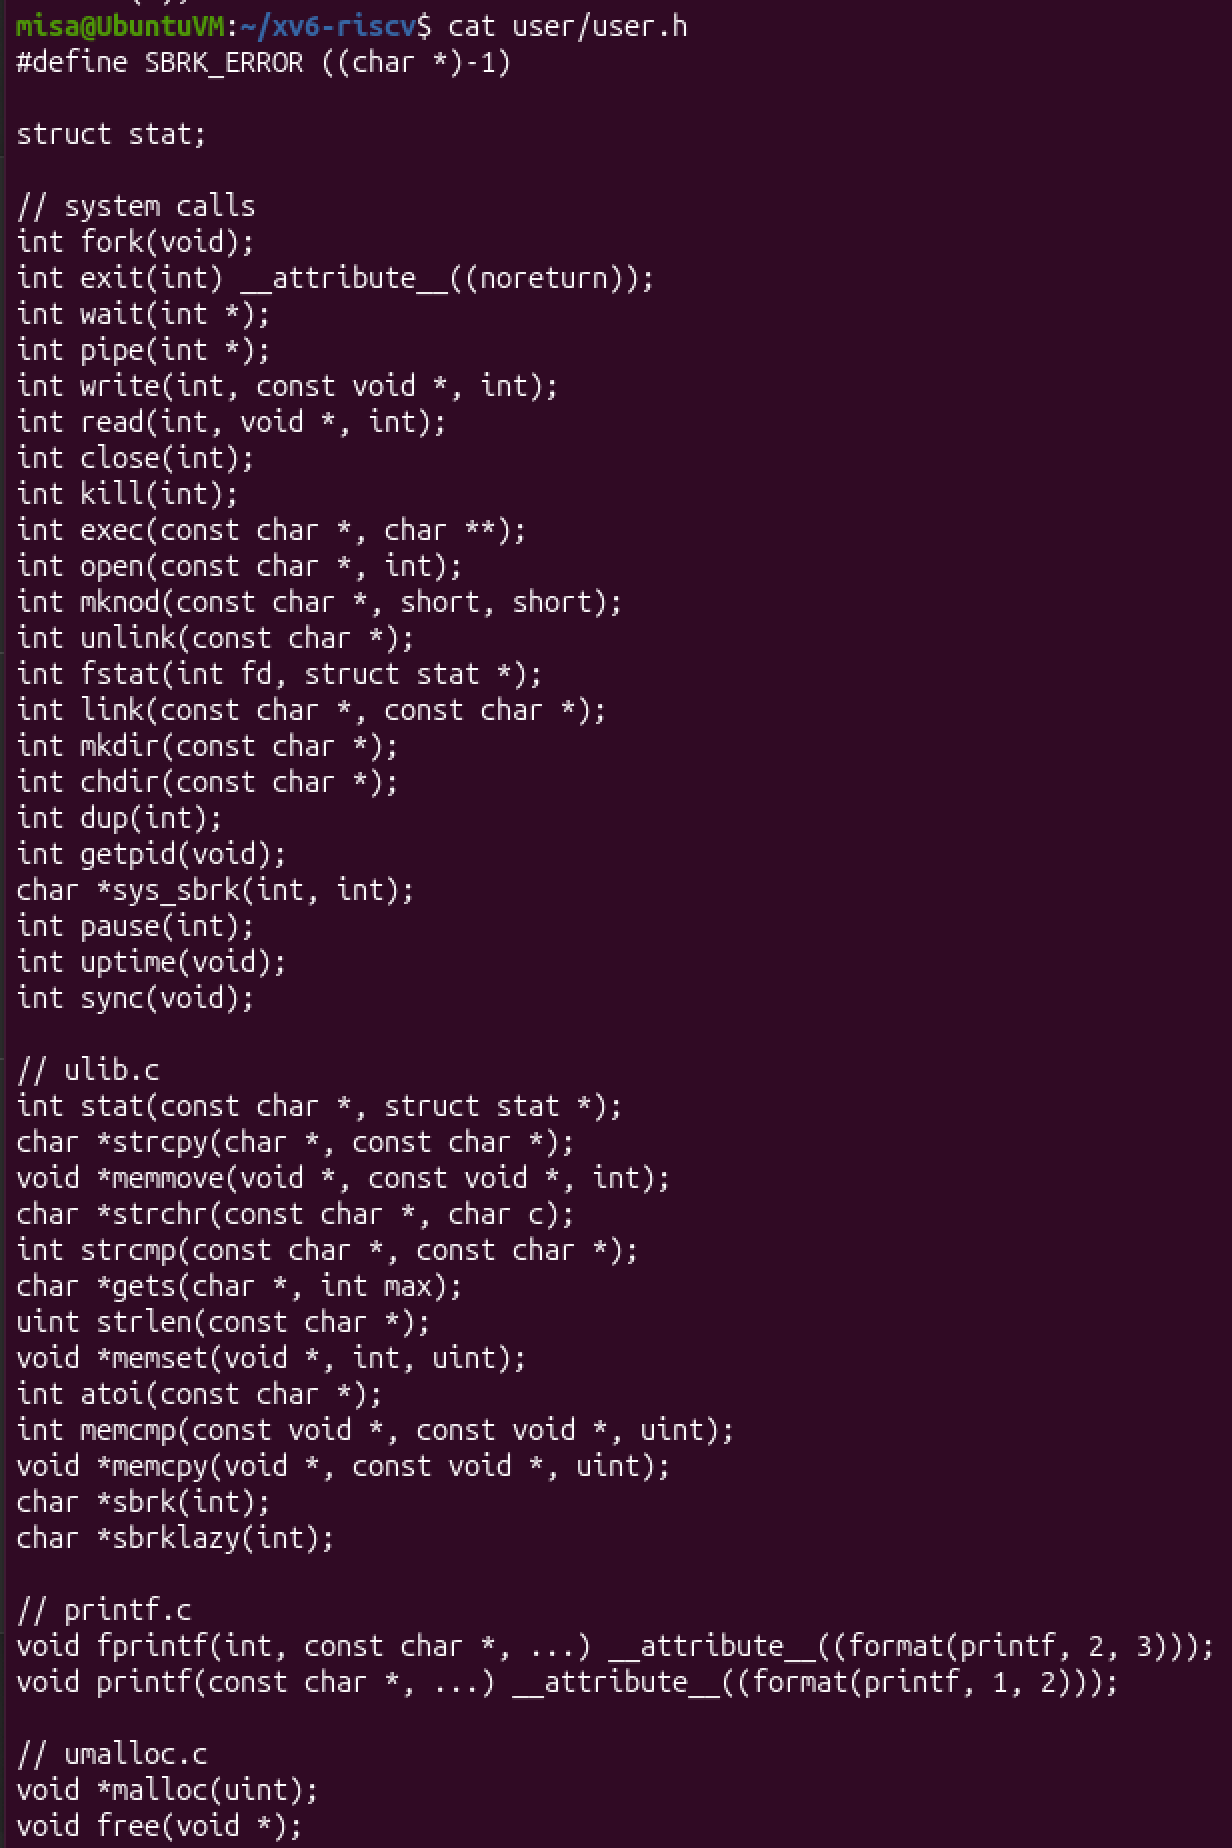
\includegraphics[width=0.82\textwidth]{./img/img_13.png}
    \caption{System call declarations in user/user.h}
    \label{fig:xv6_user_header}
\end{figure}

The corresponding kernel-side implementations of the
file-related system calls are located in
\texttt{kernel/sysfile.c}.

The \texttt{grep} command was used to locate the
\texttt{sys\_read} and \texttt{sys\_write} functions.
The option \texttt{-n} includes line numbers in the
output, while the pattern
\texttt{sys\_read\textbackslash|sys\_write}
matches either function name.

The output is passed through \texttt{head}, which
displays the first ten lines by default.

The results locate \texttt{sys\_read()} at line 69
and \texttt{sys\_write()} at line 83 of
\texttt{kernel/sysfile.c}.

\begin{figure}[H]
    \centering
    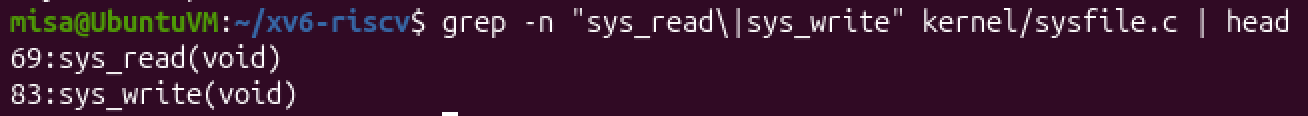
\includegraphics[width=0.82\textwidth]{./img/img_14.png}
    \caption{Locating read and write system call handlers in the kernel}
    \label{fig:xv6_syscalls}
\end{figure}

The source code demonstrates how user-space programs
access operating system services through system calls.
The user program requests an operation, while the kernel
performs it using its privileged access to system resources.


\subsection{Observations}

\begin{enumerate}
    \item \textbf{Which system calls does user/cat.c use,
    and what does each one ask the kernel to do?}

    The examined \texttt{cat()} function uses
    \texttt{read()} to obtain bytes from a file descriptor
    and \texttt{write()} to send those bytes to standard
    output. It also uses \texttt{exit()} to terminate the
    process when an error occurs.

    The complete program additionally uses file-related
    system calls such as \texttt{open()} and \texttt{close()}
    to access and release input files.

    \item \textbf{In which kernel file, and on which line,
    is sys\_read implemented?}

    The \texttt{sys\_read()} function is implemented in
    \texttt{kernel/sysfile.c}, beginning at line 69.

    \item \textbf{In one sentence: what is the difference
    between the code in kernel/ and the code in user/?}

    The \texttt{kernel/} directory contains privileged
    operating system code responsible for managing system
    resources, while \texttt{user/} contains ordinary
    programs that access these resources through system calls.
\end{enumerate}


\section{Write first xv6 program}

The next task is to create a user program called \texttt{sleep}, which
suspends its execution for a specified number of clock ticks.

The program is created in \texttt{user/sleep.c}. It receives command-line
arguments through \texttt{argc} and \texttt{argv}. The first argument
specifies the number of ticks, which is converted from a string to an
integer using \texttt{atoi()}.

The program checks that exactly one argument has been provided.
If the argument is missing or the number of arguments is incorrect,
\texttt{fprintf()} prints a usage message to standard error
(file descriptor 2), and \texttt{exit(1)} terminates the program.
Otherwise, the requested delay is performed, followed by
\texttt{exit(0)} to indicate successful completion.

The initial implementation followed the provided example and used the
\texttt{sleep()} system call. The source file was created and edited
using the Ubuntu terminal.

\begin{figure}[H]
    \centering
    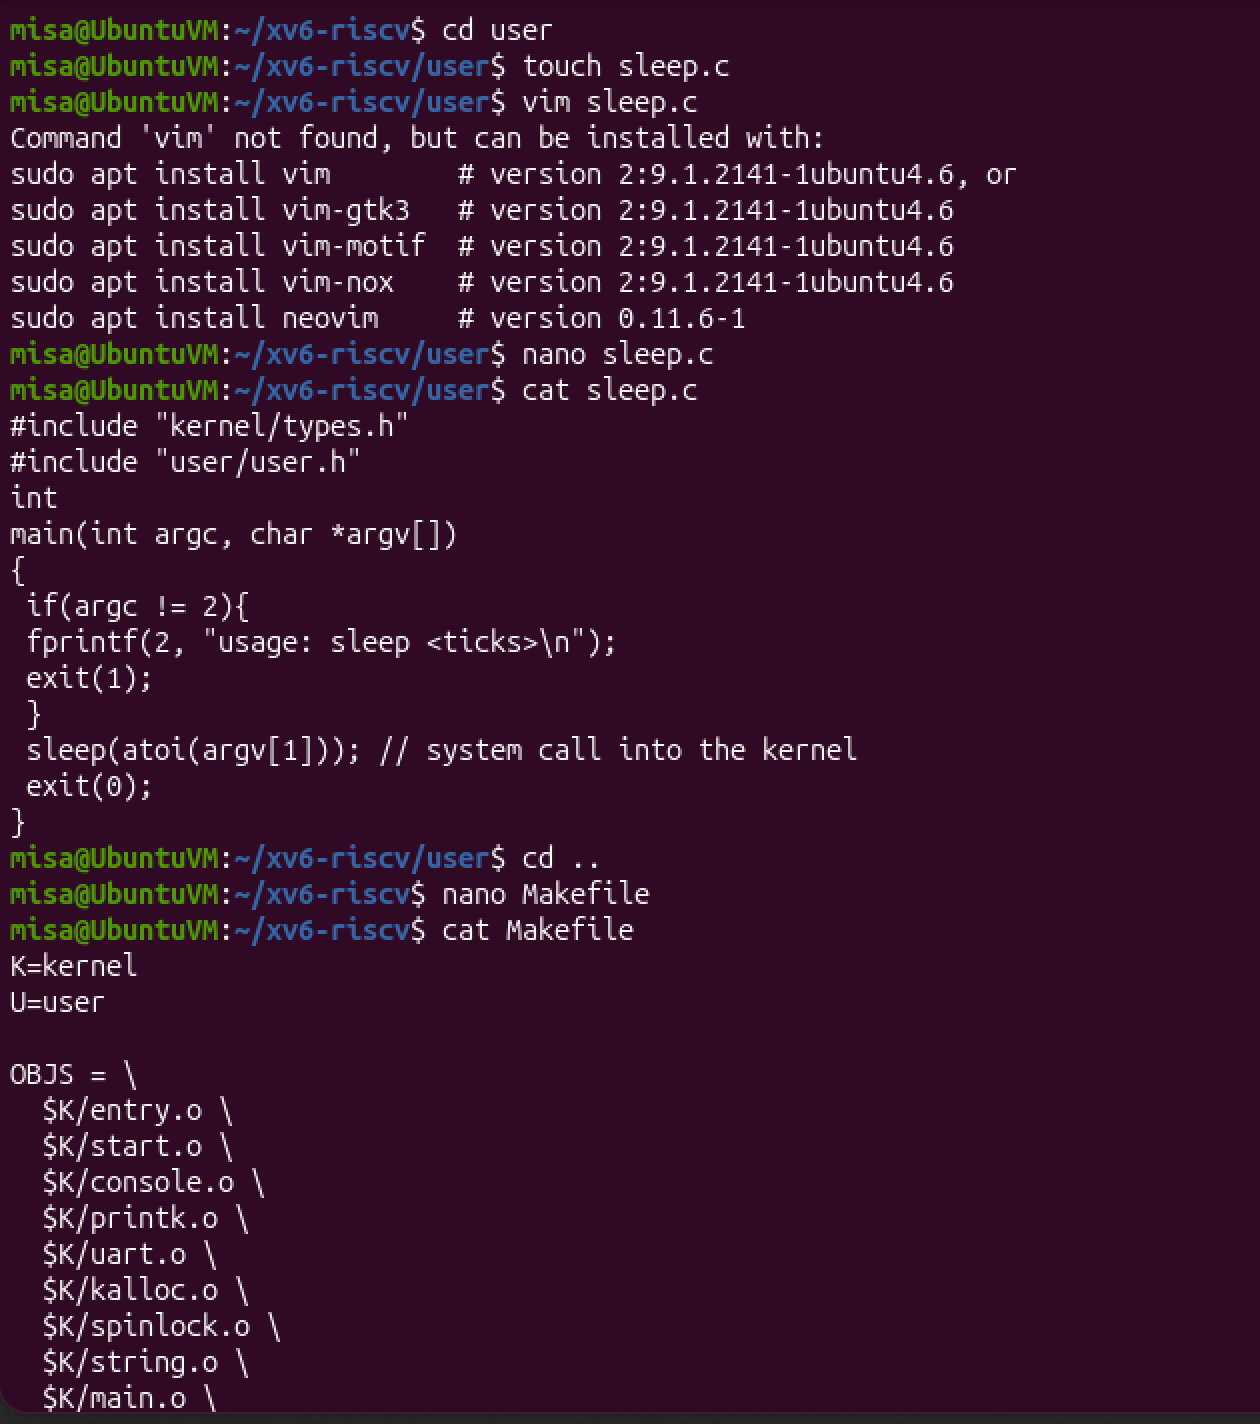
\includegraphics[width=0.82\textwidth]{./img/img_15.png}
    \caption{Creating the sleep program and inspecting its initial implementation}
    \label{fig:sleep_initial}
\end{figure}

To include the new program in the xv6 filesystem, the \texttt{UPROGS}
variable in the \texttt{Makefile} was modified by adding
\texttt{\$U/\_sleep}. This allows Make to compile and link the
program and include its executable in the filesystem image.

\begin{figure}[H]
    \centering
    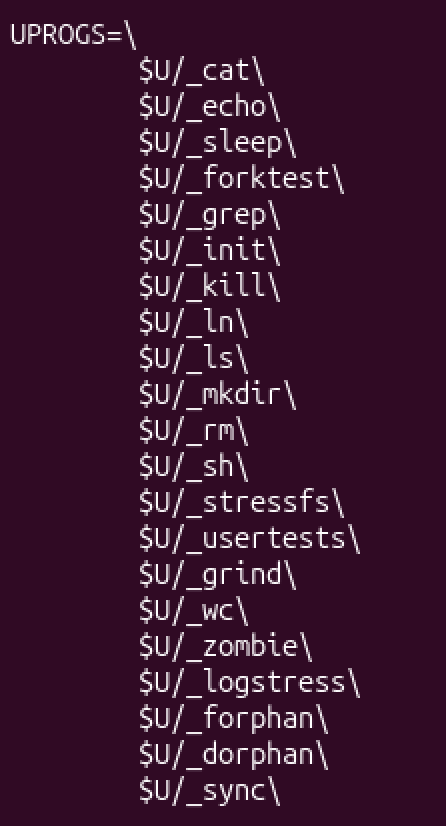
\includegraphics[width=0.82\textwidth]{./img/img_16.png}
    \caption{Registering the sleep program in the Makefile}
    \label{fig:sleep_makefile}
\end{figure}

During the first compilation attempt, GCC reported an implicit
declaration of the \texttt{sleep()} function. The current xv6
source tree exposes the corresponding functionality through
\texttt{pause(int)}, as declared in \texttt{user/user.h}.

The implementation was corrected by replacing the call to
\texttt{sleep()} with \texttt{pause()}, while preserving
the program name and its command-line interface.

The \texttt{pause()} system call suspends the calling process
for the specified number of clock ticks. The argument is passed
through \texttt{atoi(argv[1])}, allowing the user to specify
the delay directly from the shell.

\begin{figure}[H]
    \centering
    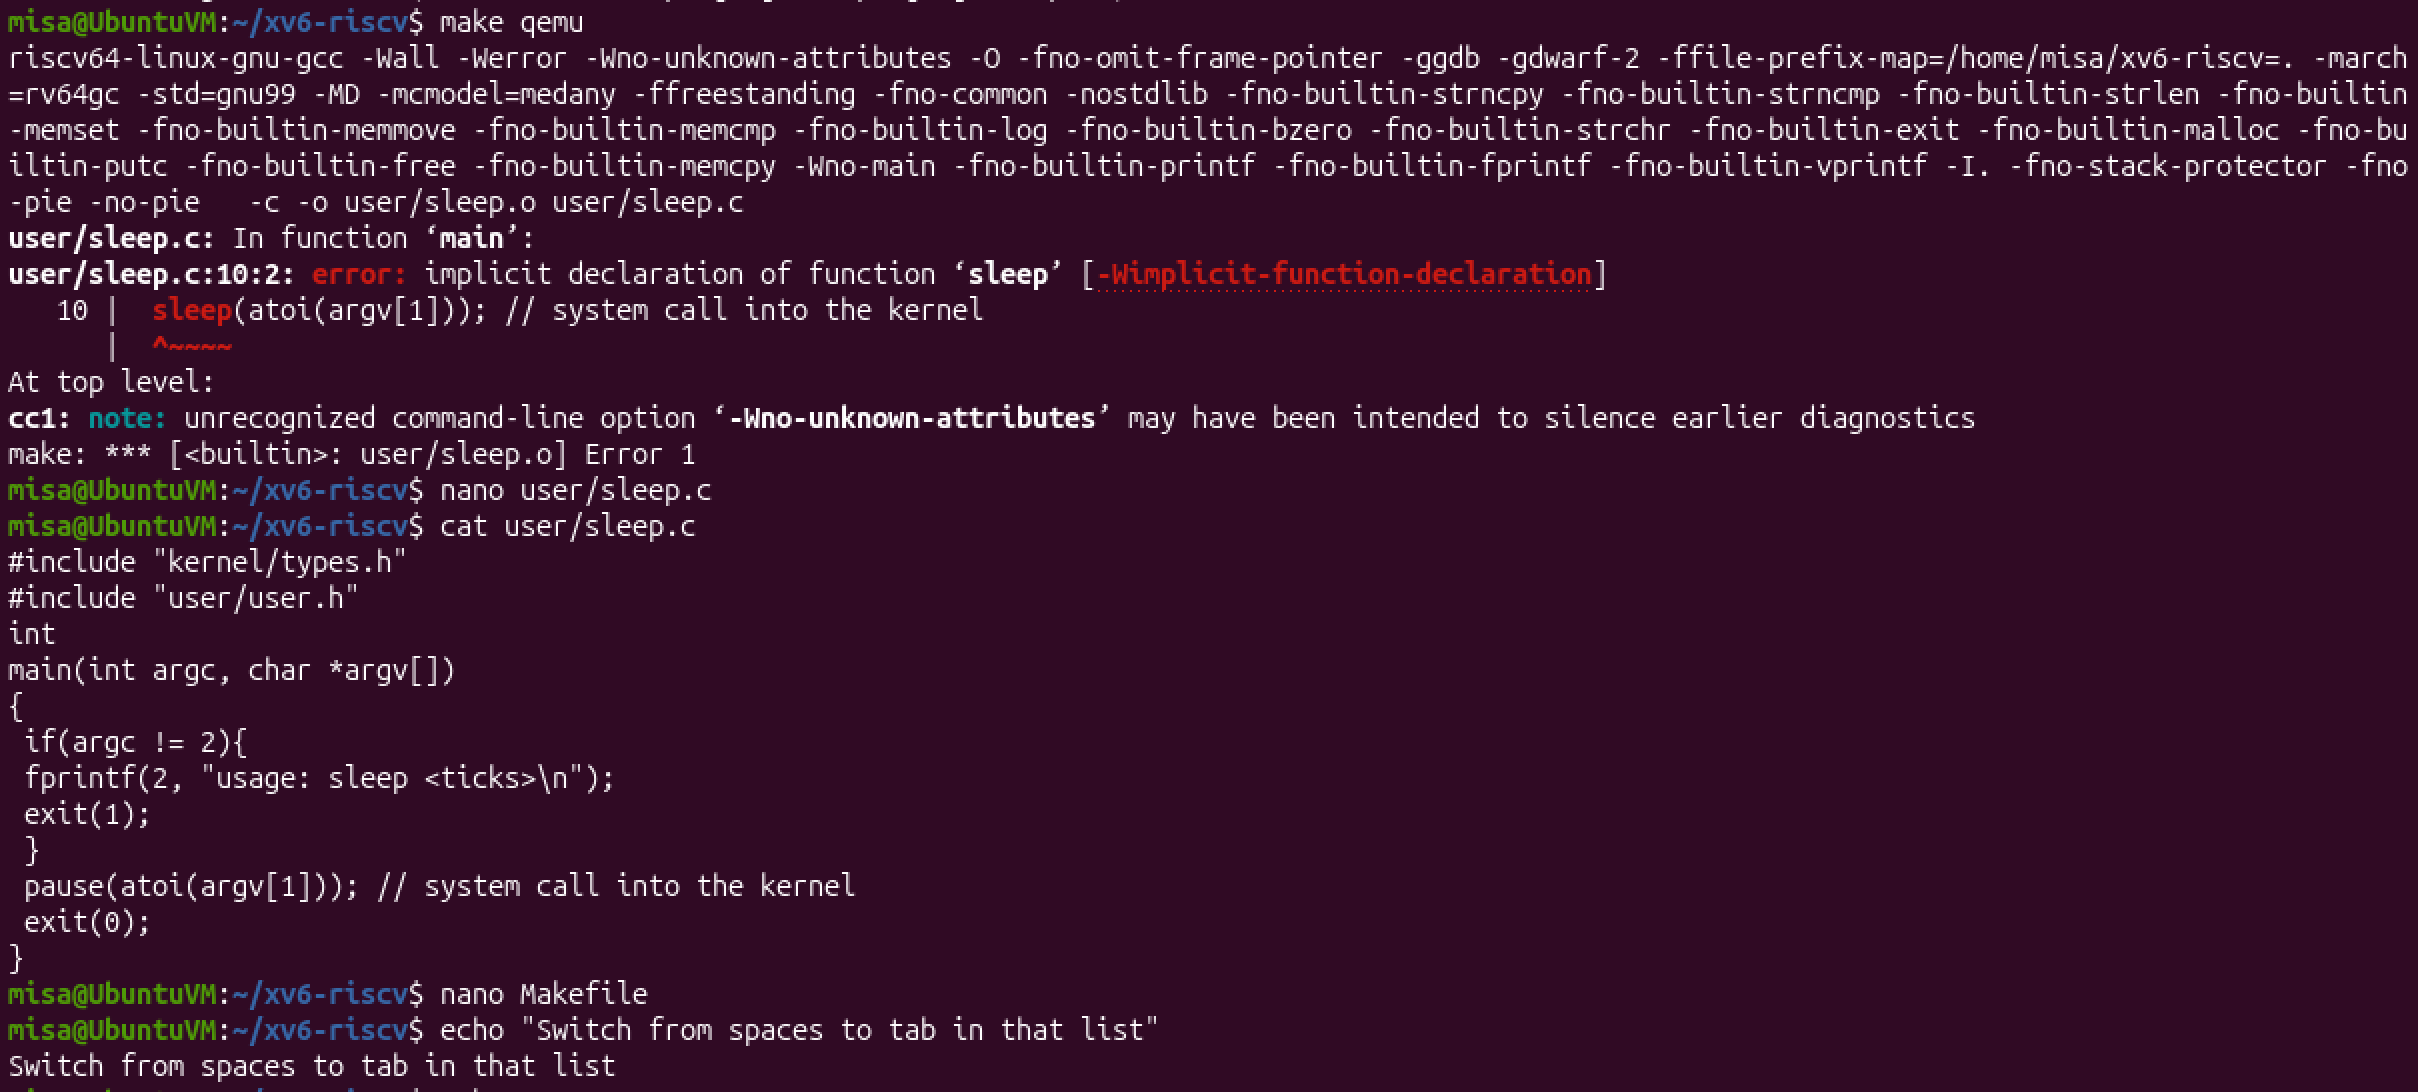
\includegraphics[width=0.82\textwidth]{./img/img_17.png}
    \caption{Compilation error and correction of the sleep system call}
    \label{fig:sleep_correction}
\end{figure}

After correcting the source code and adjusting the Makefile,
the operating system was rebuilt using \texttt{make qemu}.

The build process compiled \texttt{user/sleep.c} into
\texttt{user/sleep.o}, linked the resulting object file
into the executable \texttt{user/\_sleep}, and regenerated
the filesystem image containing the new program.

The operating system then booted successfully in QEMU.

The program was tested with two commands. Executing
\texttt{sleep 10} suspended the process for ten clock ticks
before returning control to the shell.

Executing \texttt{sleep} without an argument triggered
the argument validation and produced the expected message:
\texttt{usage: sleep <ticks>}.

\begin{figure}[H]
    \centering
    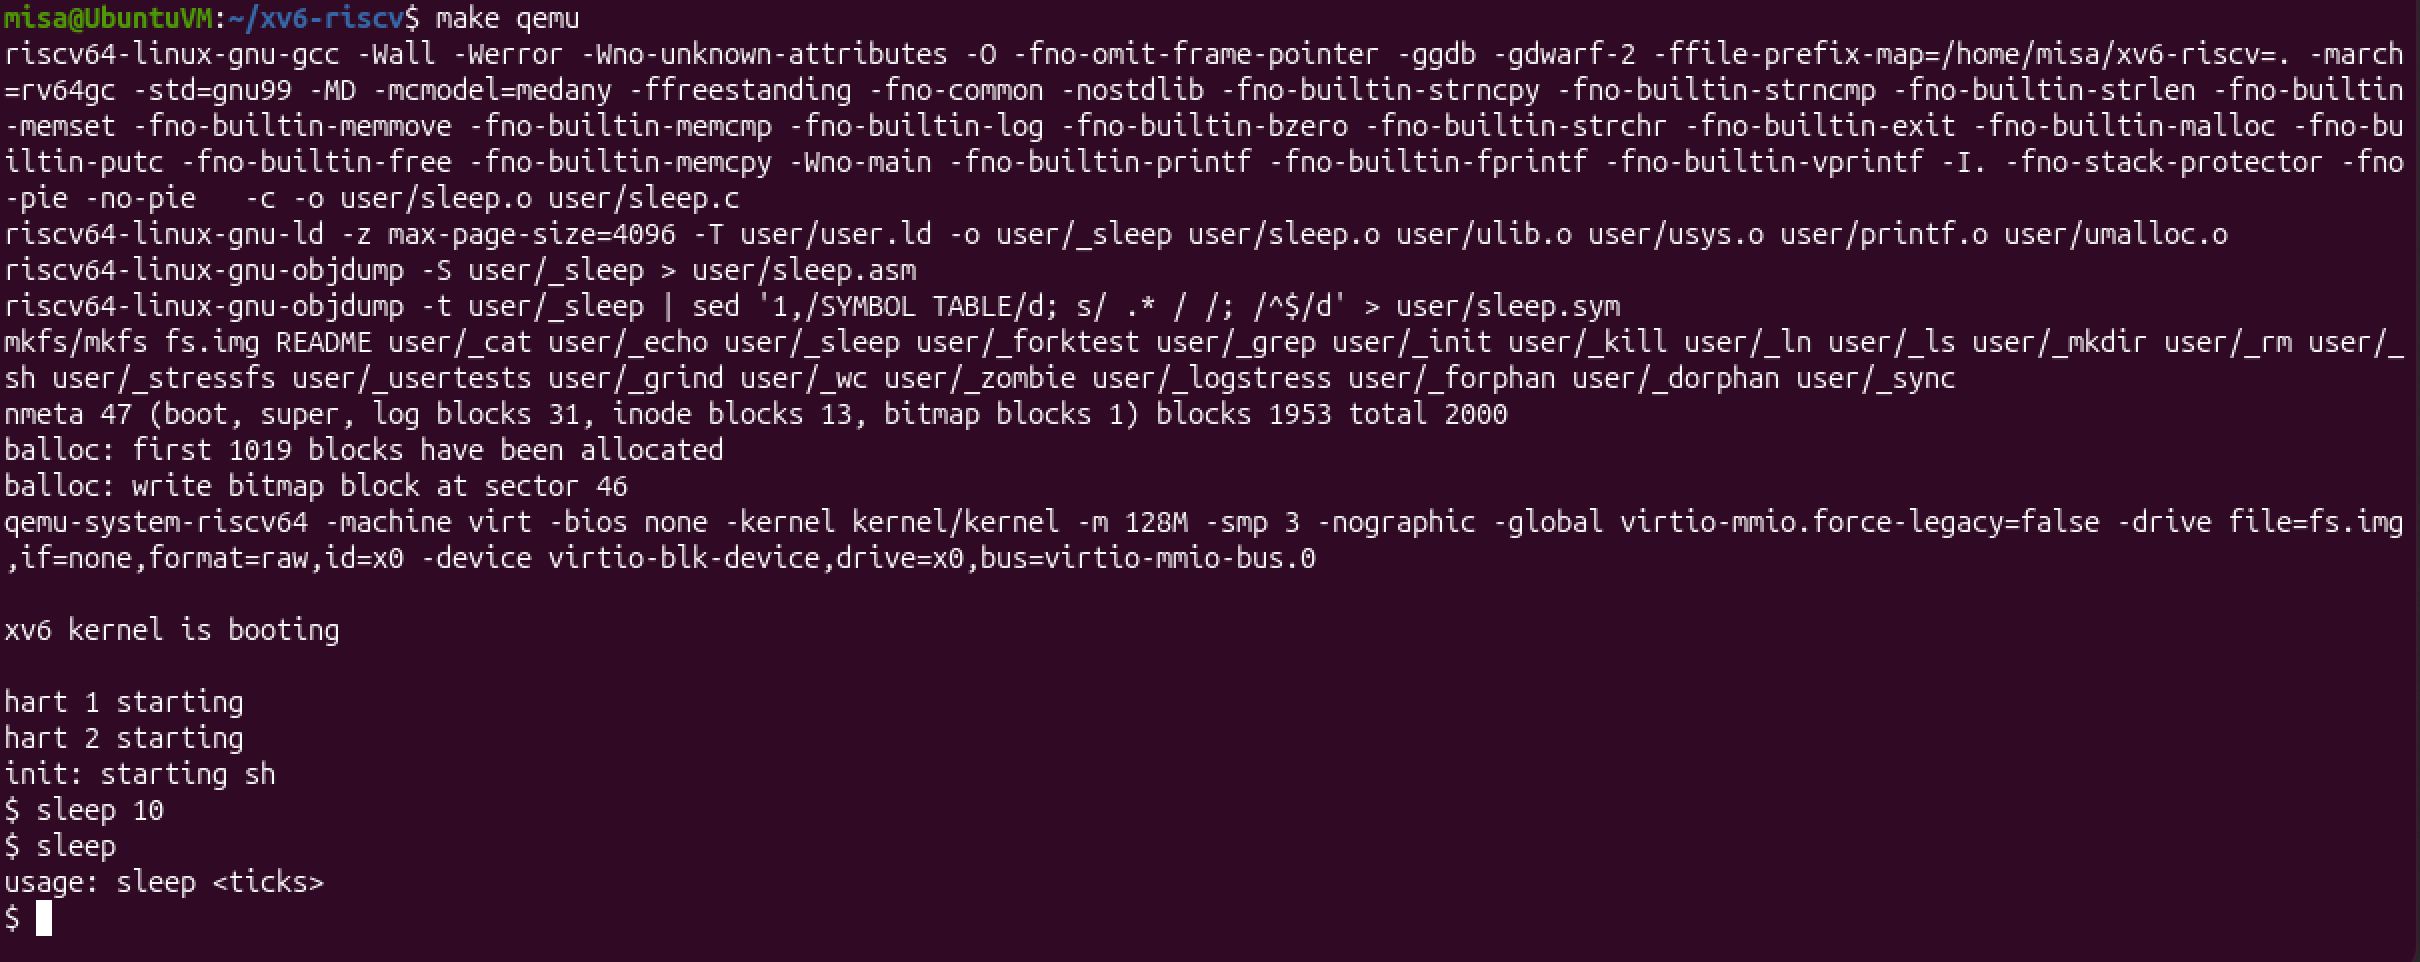
\includegraphics[width=0.82\textwidth]{./img/img_18.png}
    \caption{Successful compilation and execution of the sleep program}
    \label{fig:sleep_success}
\end{figure}

Both tests produced the expected results. The new user program
was successfully integrated into xv6 and executed using an
existing kernel system call.





\clearpage

% =======================================================================
% =======================================================================
\chapter{CONCLUSIONS}
% =======================================================================

During this laboratory work, the xv6 operating system was successfully
built from source and executed using the QEMU RISC-V emulator. The
development environment was prepared by installing the required
cross-compilation tools, and the xv6 source code was obtained from
the official repository.

Working with the xv6 shell demonstrated the basic functionality of
a Unix-like operating system, including file operations, process
execution, and inter-process communication through pipes. The system
also passed the complete user test suite, confirming the successful
execution of its kernel functionality tests.

Examining the source code provided a clearer understanding of the
separation between user-space programs and the operating system kernel.
The implementations of \texttt{ls} and \texttt{cat} demonstrated how
ordinary programs interact with system resources through system calls
such as \texttt{read()} and \texttt{write()}.

Finally, a new user program, \texttt{sleep}, was implemented and
integrated into the xv6 build process. An incompatibility between
the provided example and the current xv6 version was identified
and resolved by using \texttt{pause()} instead of \texttt{sleep()}.
After rebuilding the system, the program executed successfully
and handled both valid and missing command-line arguments.

Overall, the work provided practical experience with building,
running, examining, and extending an operating system. Working
directly with both user programs and kernel interfaces helped
establish a better understanding of how operating system
components cooperate to execute programs and provide services.
% =======================================================================


% =======================================================================
% =======================================================================


\clearpage

% =======================================================================
% Bibliography
% =======================================================================

%\begin{thebibliography}{99}
\singlespace \normalsize

% \bibitem{ref:Chicago}
%   The Chicago Manual of Style.
%   "Notes and Bibliography: Sample Citations".
%   Accessed October 14, 2022.
%   \url{https://www.chicagomanualofstyle.org/tools_citationguide/citation-guide-2.html}.

% \bibitem{ref:Cats}
%   Google.
%   "Search results for cats".
%   Accessed August 15, 2023.
%   \url{https://www.google.com/search?q=cats}.

\bibitem{ref:OS-GfG}
  GeeksforGeeks.
  "What is an Operating System?".
  Last Updated July 25, 2025.
  Accessed October 16, 2025.
  \url{https://www.geeksforgeeks.org/operating-systems/what-is-an-operating-system/}.

\bibitem{ref:OS-concept}
Silberschatz, A., Galvin, P. B., \& Gagne, G. (2018).
\textit{Operating System Concepts} (10th ed.).
Wiley.
ISBN 978-1-119-32091-3.

\end{thebibliography}



\clearpage
\end{document}
